% Options for packages loaded elsewhere
\PassOptionsToPackage{unicode,linktoc=all}{hyperref}
\PassOptionsToPackage{hyphens}{url}
\PassOptionsToPackage{dvipsnames,svgnames,x11names}{xcolor}
%
\documentclass[
  a4paper,
]{article}
\usepackage{amsmath,amssymb}
\usepackage{iftex}
\ifPDFTeX
  \usepackage[T1]{fontenc}
  \usepackage[utf8]{inputenc}
  \usepackage{textcomp} % provide euro and other symbols
\else % if luatex or xetex
  \usepackage{unicode-math} % this also loads fontspec
  \defaultfontfeatures{Scale=MatchLowercase}
  \defaultfontfeatures[\rmfamily]{Ligatures=TeX,Scale=1}
\fi
\usepackage{lmodern}
\ifPDFTeX\else
  % xetex/luatex font selection
\fi
% Use upquote if available, for straight quotes in verbatim environments
\IfFileExists{upquote.sty}{\usepackage{upquote}}{}
\IfFileExists{microtype.sty}{% use microtype if available
  \usepackage[]{microtype}
  \UseMicrotypeSet[protrusion]{basicmath} % disable protrusion for tt fonts
}{}
\makeatletter
\@ifundefined{KOMAClassName}{% if non-KOMA class
  \IfFileExists{parskip.sty}{%
    \usepackage{parskip}
  }{% else
    \setlength{\parindent}{0pt}
    \setlength{\parskip}{6pt plus 2pt minus 1pt}}
}{% if KOMA class
  \KOMAoptions{parskip=half}}
\makeatother
\usepackage{xcolor}
\usepackage[margin=25mm]{geometry}
\usepackage{longtable,booktabs,array}
\usepackage{calc} % for calculating minipage widths
% Correct order of tables after \paragraph or \subparagraph
\usepackage{etoolbox}
\makeatletter
\patchcmd\longtable{\par}{\if@noskipsec\mbox{}\fi\par}{}{}
\makeatother
% Allow footnotes in longtable head/foot
\IfFileExists{footnotehyper.sty}{\usepackage{footnotehyper}}{\usepackage{footnote}}
\makesavenoteenv{longtable}
\usepackage{graphicx}
\makeatletter
\def\maxwidth{\ifdim\Gin@nat@width>\linewidth\linewidth\else\Gin@nat@width\fi}
\def\maxheight{\ifdim\Gin@nat@height>\textheight\textheight\else\Gin@nat@height\fi}
\makeatother
% Scale images if necessary, so that they will not overflow the page
% margins by default, and it is still possible to overwrite the defaults
% using explicit options in \includegraphics[width, height, ...]{}
\setkeys{Gin}{width=\maxwidth,height=\maxheight,keepaspectratio}
% Set default figure placement to htbp
\makeatletter
\def\fps@figure{htbp}
\makeatother
\setlength{\emergencystretch}{3em} % prevent overfull lines
\providecommand{\tightlist}{%
  \setlength{\itemsep}{0pt}\setlength{\parskip}{0pt}}
\setcounter{secnumdepth}{-\maxdimen} % remove section numbering
\ifLuaTeX
\usepackage[bidi=basic]{babel}
\else
\usepackage[bidi=default]{babel}
\fi
\babelprovide[main,import]{british}
% get rid of language-specific shorthands (see #6817):
\let\LanguageShortHands\languageshorthands
\def\languageshorthands#1{}
% $HOME/.pandoc/defaults/latex-header-includes.tex
% Common header includes for both lualatex and xelatex engines.
%
% Preliminaries
%
% \PassOptionsToPackage{rgb,dvipsnames,svgnames}{xcolor}
% \PassOptionsToPackage{main=british}{babel}
\PassOptionsToPackage{english}{selnolig}
\AtBeginEnvironment{quote}{\small}
\AtBeginEnvironment{quotation}{\small}
\AtBeginEnvironment{longtable}{\centering}
%
% Packages that are useful to include
%
\usepackage{graphicx}
\usepackage{subcaption}
\usepackage[inkscapeversion=1]{svg}
\usepackage[defaultlines=4,all]{nowidow}
\usepackage{etoolbox}
\usepackage{fontsize}
\usepackage{newunicodechar}
\usepackage{pdflscape}
\usepackage{fnpct}
\usepackage{parskip}
  \setlength{\parindent}{0pt}
\usepackage[style=american]{csquotes}
% \usepackage{setspace} Use the <fontname-plus.tex> files for setspace
%
\usepackage{esdiff} % for derivative symbols
\usepackage{amsmath}
\usepackage{hyperref} % cleveref must come AFTER hyperref
\usepackage[capitalize,noabbrev]{cleveref} % Must come after hyperref
% noto-plus.tex
% Font-setting header file for use with Pandoc Markdown
% to generate PDF via LuaLaTeX.
% The main font is Noto Serif.
% Other main fonts are also available in appropriately named file.
\usepackage{fontspec}
\usepackage{setspace}
\setstretch{1.3}
%
\defaultfontfeatures{Ligatures=TeX,Scale=MatchLowercase,Renderer=Node} % at the start always
%
% For English
% See also https://tex.stackexchange.com/questions/574047/lualatex-amsthm-polyglossia-charissil-error
% We use Node as Renderer for the Latin Font and Greek Font and HarfBuzz as renderer ofr Indic fonts.
%
\babelfont{rm}[Script=Latin,Scale=1]{NotoSerif}% Config is at $HOME/texmf/tex/latex/NotoSerif.fontspec
%
\babelfont{sf}[Script=Latin]{SourceSansPro}% Config is at $HOME/texmf/tex/latex/SourceSansPro.fontspec
%
\babelfont{tt}[Script=Latin]{FiraMono}% Config is at $HOME/texmf/tex/latex/FiraMono.fontspec
%
% Sanskrit, Tamil, and Greek fonts
%
\babelprovide[import, onchar=ids fonts]{sanskrit}
\babelprovide[import, onchar=ids fonts]{tamil}
\babelprovide[import, onchar=ids fonts]{greek}
%
\babelfont[sanskrit]{rm}[Scale=1.1,Renderer=HarfBuzz,Script=Devanagari]{NotoSerifDevanagari}
\babelfont[sanskrit]{sf}[Scale=1.1,Renderer=HarfBuzz,Script=Devanagari]{NotoSansDevanagari}
\babelfont[tamil]{rm}[Renderer=HarfBuzz,Script=Tamil]{NotoSerifTamil}
\babelfont[tamil]{sf}[Renderer=HarfBuzz,Script=Tamil]{NotoSansTamil}
\babelfont[greek]{rm}[Script=Greek]{GentiumBookPlus}
%
% Math font
%
\usepackage{unicode-math} % seems not to hurt % fallabck
\setmathfont[bold-style=TeX]{STIX Two Math}
%
%
% Other fonts
%
\newfontfamily{\emojifont}{Symbola}
%

\usepackage{titling}
\usepackage{fancyhdr}
    \pagestyle{fancy}
    \fancyhead{}
    \fancyfoot{}
    \renewcommand{\headrulewidth}{0.2pt}
    \renewcommand{\footrulewidth}{0.2pt}
    \fancyhead[LO,RE]{\scshape\thetitle}
    \fancyfoot[CO,CE]{\footnotesize Copyright © 2006\textendash\the\year, R (Chandra) Chandrasekhar}
    \fancyfoot[RE,RO]{\thepage}
\newfontfamily{\regulariconfont}{Font Awesome 6 Free Regular}[Color=Grey]
\newfontfamily{\solidiconfont}{Font Awesome 6 Free Solid}[Color=Grey]
\newfontfamily{\brandsiconfont}{Font Awesome 6 Brands}[Color=Grey]
%
% Direct input of Unicode code points
%
\newcommand{\faEnvelope}{\regulariconfont\ ^^^^f0e0\normalfont}
\newcommand{\faMobile}{\solidiconfont\ ^^^^f3cd\normalfont}
\newcommand{\faLinkedin}{\brandsiconfont\ ^^^^f0e1\normalfont}
\newcommand{\faGithub}{\brandsiconfont\ ^^^^f09b\normalfont}
\newcommand{\faAtom}{\solidiconfont\ ^^^^f5d2\normalfont}
\newcommand{\faPaperPlaneRegular}{\regulariconfont\ ^^^^f1d8\normalfont}
\newcommand{\faPaperPlaneSolid}{\solidiconfont\ ^^^^f1d8\normalfont}

%
% The block below is commented out because of Tofu glyphs in HTML
%
% \newcommand{\faEnvelope}{\regulariconfont\ \normalfont}
% \newcommand{\faMobile}{\solidiconfont\ \normalfont}
% \newcommand{\faLinkedin}{\brandsiconfont\ \normalfont}
% \newcommand{\faGithub}{\brandsiconfont\ \normalfont}
\ifLuaTeX
  \usepackage{selnolig}  % disable illegal ligatures
\fi
\IfFileExists{bookmark.sty}{\usepackage{bookmark}}{\usepackage{hyperref}}
\IfFileExists{xurl.sty}{\usepackage{xurl}}{} % add URL line breaks if available
\urlstyle{sf}
\hypersetup{
  pdftitle={Varieties of Multiplication},
  pdfauthor={R (Chandra) Chandrasekhar},
  pdflang={en-GB},
  colorlinks=true,
  linkcolor={DarkOliveGreen},
  filecolor={Purple},
  citecolor={DarkKhaki},
  urlcolor={Maroon},
  pdfcreator={LaTeX via pandoc}}

\title{Varieties of Multiplication}
\author{R (Chandra) Chandrasekhar}
\date{2012-05-14 | 2023-11-10}

\begin{document}
\maketitle

\thispagestyle{empty}


\begin{quote}
This was my first blog---written in 2012---under the
\href{https://swanlotus.netlify.app/tag/mathematical-musings}{\emph{Mathemtical
Musings}} tag. The intention was to re-visit topics in mathematics that
trigger concern or disquiet in the earnest student of the subject. My
hope was that ideas that appeared puzzling or forbidding at first sight
could be coaxed to become friendly and helpful. Unhurried explanations
and a different perspective would underpin the approach. I have
retained, substantially unchanged, what I first wrote, to maintain the
freshness, flavour, and vintage of the original blog, even if it is a
little rough around the edges.
\end{quote}

\hypertarget{prologue}{%
\subsection{Prologue}\label{prologue}}

This blog is experimental in three ways.

First, this is my maiden attempt to display mathematics on a web page.
It might look simple, but believe me, it is no mean task. Thanks to the
concerted efforts of many generous people, I am using
\href{https://www.mathjax.org/}{MathJax} to render the mathematics via
\href{https://pandoc.org/}{Pandoc}, and its flavour of
\href{https://garrettgman.github.io/rmarkdown/authoring_pandoc_markdown.html}{Markdown}.

The second experimental feature is what I have called ``slicing the
orange of knowledge with a different cut'' in my book
\href{https://swanlotus.netlify.app/sas}{\emph{Secrets of Academic
Success}}. The idea of multiplication runs like a thread through much of
mathematics, from the most elementary stages of counting to what
constitutes cutting edge research. Unfortunately, in the way mathematics
is taught at present, multiplication is bundled with each stage of
mathematics and viewed separately as an operation in that context.

By concentrating on the single unifying \emph{idea} of multiplication,
and viewing it across the whole of mathematics, we are indeed ``slicing
the orange of knowledge with a different cut''. Even if you have not
encountered some of the varieties of multiplication mentioned here, this
exposure will help you grasp those varieties better when you do
encounter them. Please \href{mailto:feedback.swanlotus@gmail.com}{send
me feedback} on whether this approach works for you.

Third, this is an \emph{extremely long} blog. In fact, I call it a
\href{https://www.vocabulary.com/dictionary/slog}{\emph{slog}}
\emojifont {😉} \normalfont. It took me some weeks to write it. So, take
your time reading it. It is unlikely that you will finish it at one
sitting. \emph{Read it in parts at your own pace}. After having read it
once, cast your eyes and mind over the whole to get an overall view of
the main ideas.

I thought of splitting the blog into three or four manageable parts, but
decided against it because I wanted the evolution of multiplication as
an idea to be left whole in a single post.
\href{mailto:feedback.swanlotus@gmail.com}{Tell me} if it put you to
sleep \emojifont {😄} \normalfont.

With that out of the way, let us begin. I want to look at some of the
varieties of multiplication that mathematicians have developed over
time. It is a survey that will serve as a pinhole through which we can
view how a single, simple mathematical idea has been expanded and
elaborated into uses far beyond its historical moorings.

\hypertarget{multiplication-as-a-binary-operation}{%
\subsection{Multiplication as a binary
operation}\label{multiplication-as-a-binary-operation}}

Consistency is valued more in mathematics than in other disciplines.
\emph{The idea is not to upset the apple cart but to expand it}.
Definitions, conventions, rules, facts, and fallacies---once
established---are usually above argument, and do not vary with time or
place. So, let us start by defining some terms.

Multiplication is a \emph{binary} operation: it is something that we do
with \emph{two} mathematical objects, whatever they might be. Usually,
the two are \emph{similar} objects or at least \emph{compatible}
objects. The whole numbers are an example. We can and do multiply two
whole numbers.

\hypertarget{multiplication-as-repeated-addition}{%
\subsection{Multiplication as repeated
addition}\label{multiplication-as-repeated-addition}}

Practically and historically, multiplication arose as an arithmetic
convenience for repeated addition. If we add the number \(3\) four
times, we have \[
3 + 3 + 3 + 3 = (3 + 3) + (3 + 3) = 6 + 6 = 12
\] The reason for adding \(3\) in \emph{pairs}, as shown above, is that
addition is a binary operation, just like multiplication. Using the
shorthand of multiplication, we write this as \(4 \times 3 = 12\).
\emph{So, multiplication is a shorthand for repeated addition.}

When we see the arithmetic expression \(4 \times 3\), we say ``four
times three'' in English. Or, we could equally well say ``four threes'',
as I was taught at school, which is less ambiguous and much clearer.
Think of four lots of three being added together like we have seen
above: \begin{equation}\protect\hypertarget{eq:multiplier}{}{
\begin{array}{c c c r}
4 &\times &3 &= 3 + 3 + 3 + 3 = (3 + 3) + (3 + 3) = 6 + 6 = 12\\
\uparrow & & \uparrow & \uparrow\\
\mbox{multiplier} & & \mbox{multiplicand} & \mbox{product}\\
\end{array}
}\label{eq:multiplier}\end{equation} The number \(4\) is the
\href{https://www.thefreedictionary.com/multiplier}{multiplier} and the
number \(3\) is the
\href{https://mathworld.wolfram.com/Multiplicand.html}{multiplicand}.
This is the standard definition.

We say that the ``something'' which is repeatedly added, is the
\emph{multiplicand.} The number of times that ``something'' is added is
the \emph{multiplier.} And the result of this operation is the
\emph{product.} Thus far we are in perfect harmony with accepted usage.

\hypertarget{commutativity-and-multiplication}{%
\subsection{Commutativity and
multiplication}\label{commutativity-and-multiplication}}

Multiplication of numbers is \href{}{commutative}, i.e., the multiplier
and multiplicand can change roles without affecting the result.
\begin{equation}\protect\hypertarget{eq:comm}{}{
4 \times 3 = 3 \times 4 = 12.
}\label{eq:comm}\end{equation} Note that at the very left of
\cref{eq:comm}, \(4\) is the multiplier, and \(3\) the multiplicand,
whereas in the middle of \cref{eq:comm}, \(3\) is the multiplier and
\(4\) the multiplicand. To labour the point,
\begin{equation}\protect\hypertarget{eq:multiplicand}{}{
\begin{array}{c c c r}
3 &\times &4 &= 4 + 4 + 4 = (4 +4) + 4 = 4 + (4 + 4) = 12\\
\uparrow & & \uparrow & \uparrow\\
\mbox{multiplier} & & \mbox{multiplicand} & \mbox{product}\\
\end{array}
}\label{eq:multiplicand}\end{equation} Although the two numbers have
changed their names and roles from \cref{eq:multiplier} to
\cref{eq:multiplicand}, the result is the same because the
multiplication of numbers is commutative.

To accommodate our
\href{https://www.thefreedictionary.com/zeitgeist}{zeitgeist}, the
distinction between multiplier and multiplicand is fading away, in
favour of the symmetrical and neutral term \emph{factor}. The result of
multiplying two \emph{factors} is still the \emph{product}, as before.

\hypertarget{rectangular-numbers}{%
\subsection{Rectangular numbers}\label{rectangular-numbers}}

Historically, stones were used to count. And the stones representing any
number may be arranged in geometric shapes, like lines, triangles,
rectangles, and so on. This gives us a geometrical or pictorial
representation of numbers.

All numbers which are the products of two whole numbers, neither of
which is one, may be expressed as \emph{rectangular numbers}. The
symbolic operation \(4 \times 3\) may be shown pictorially as a series
of \(12\) icons arranged four across and three high. Because we may swap
the order of multiplication, we may also show it as \(12\) rectangles
three across and four high. As we have seen, multiplication of numbers
is commutative. The image below shows this equivalence.

\begin{figure}
\hypertarget{fig:four-by-three}{%
\centering
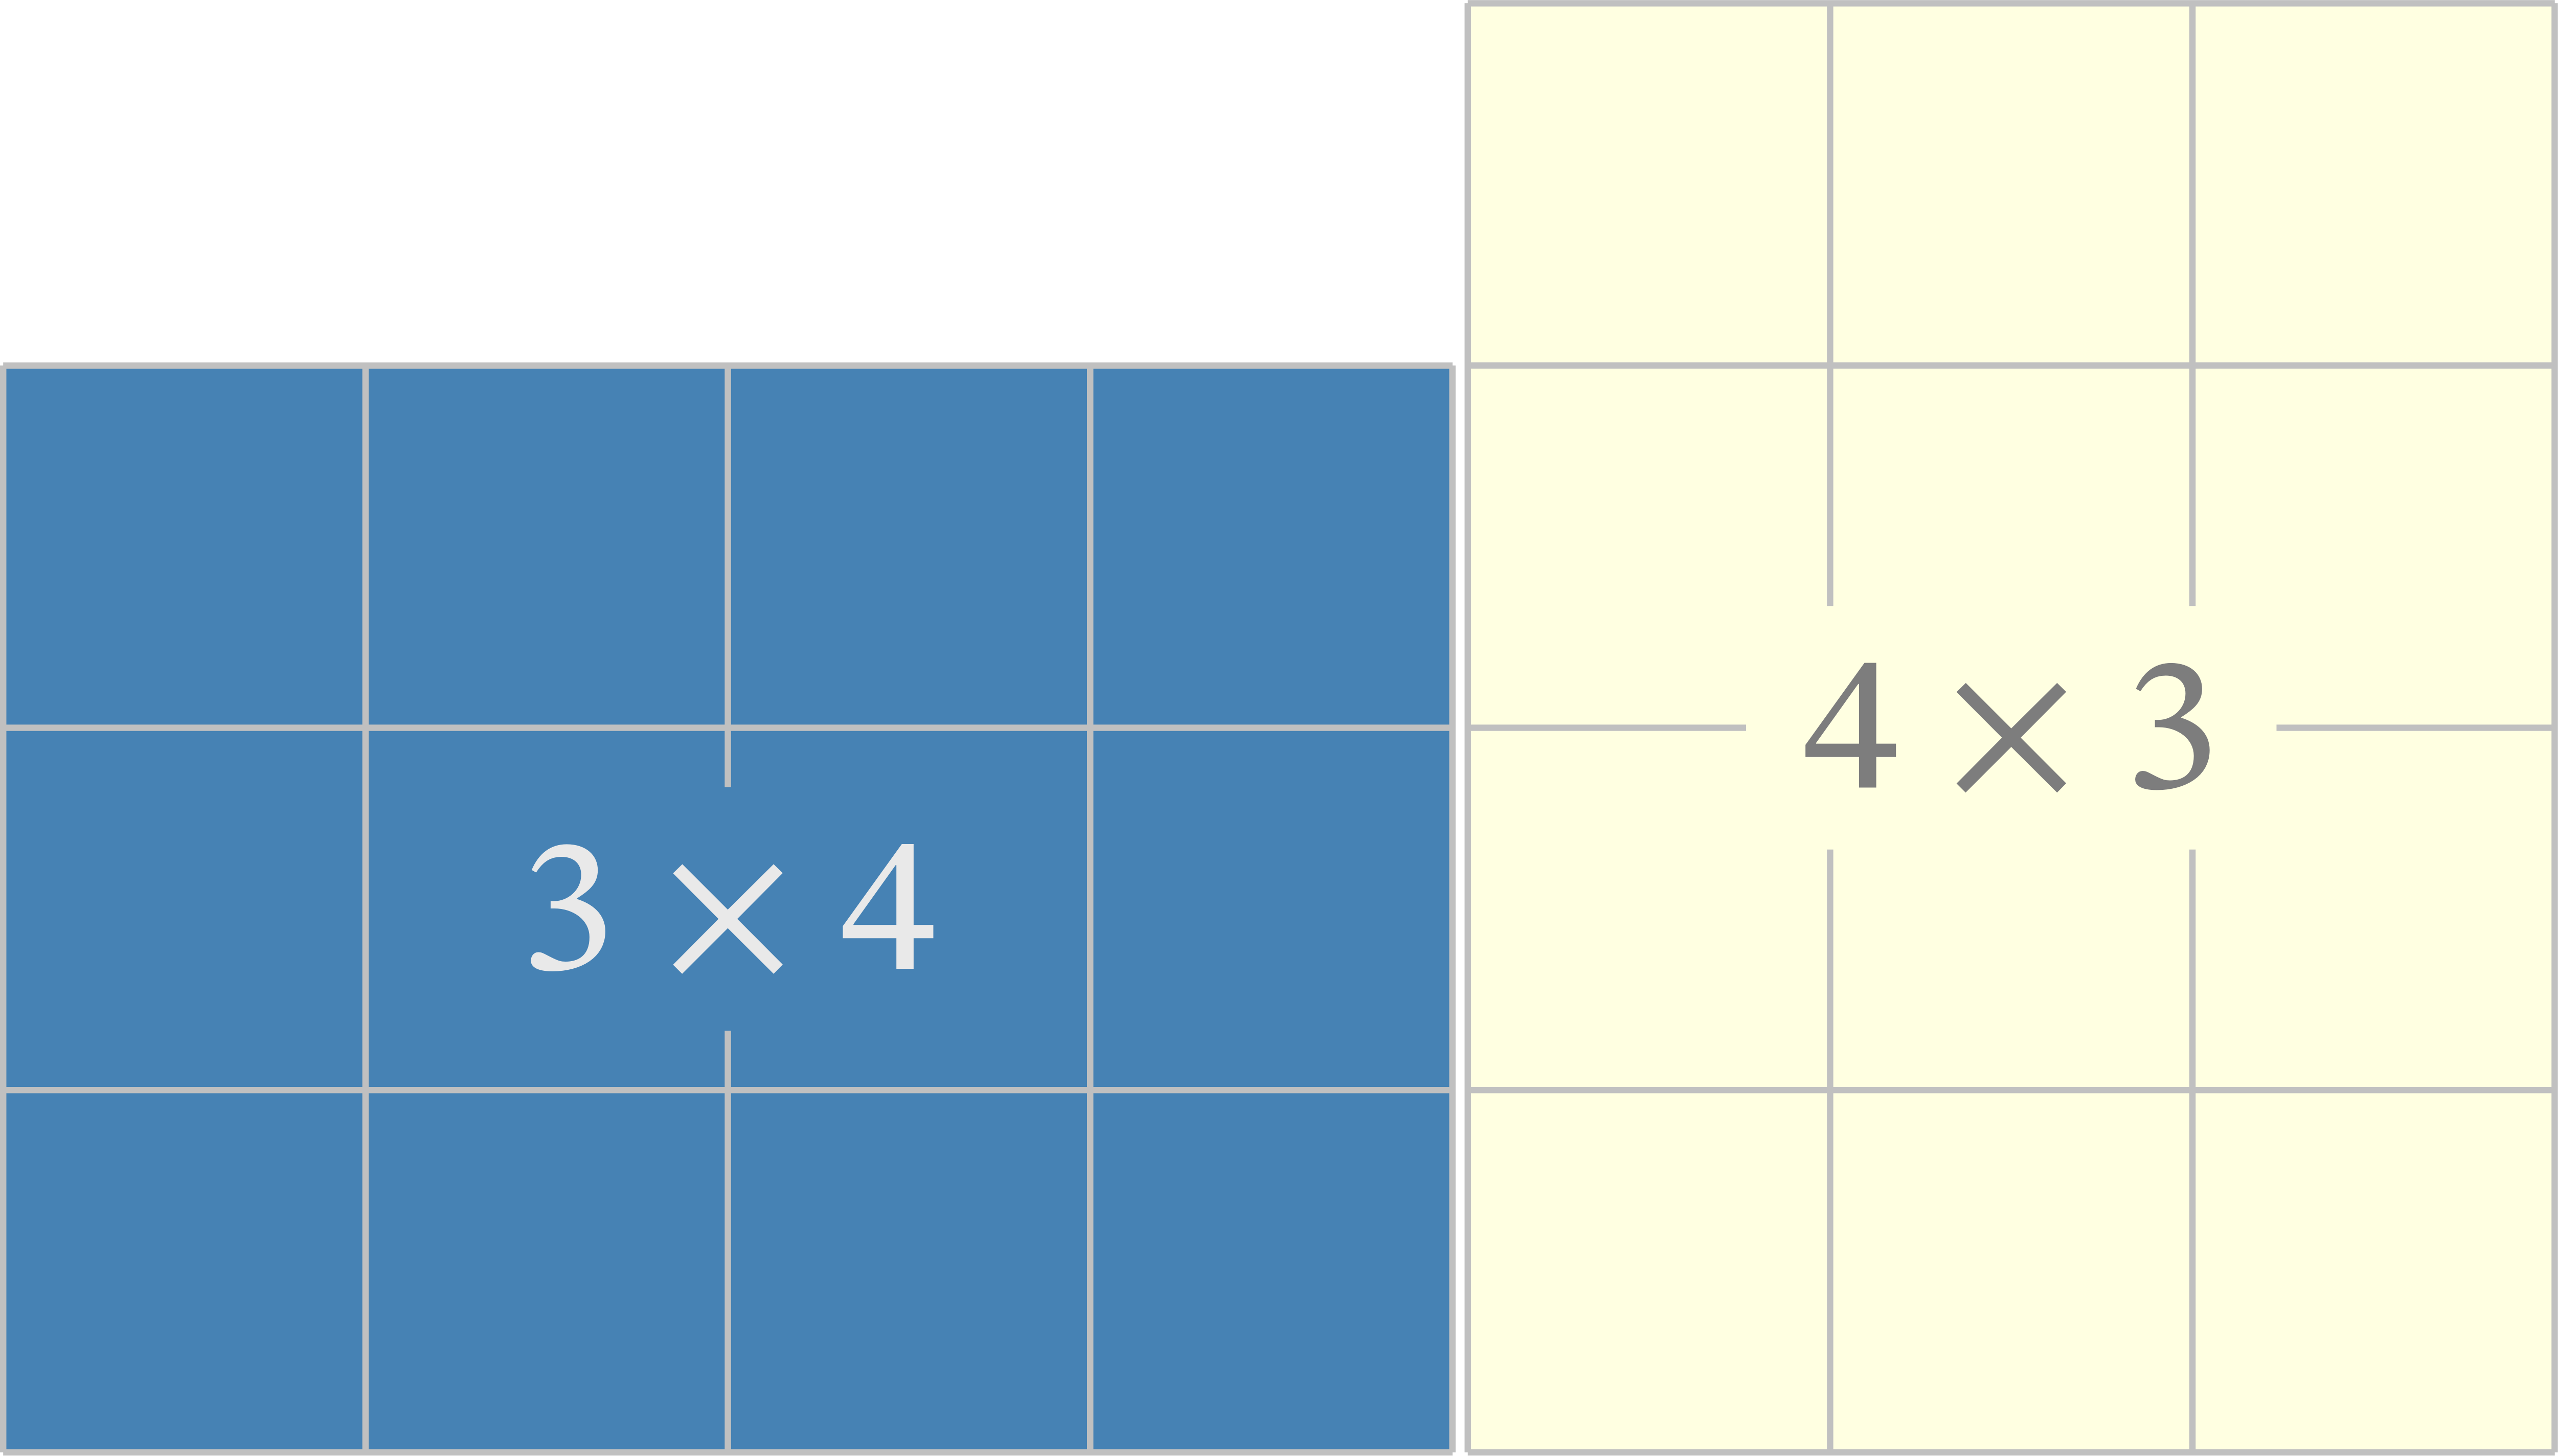
\includegraphics[width=0.5\textwidth,height=\textheight]{images/four-by-three.png}
\caption{The multiplier is the number of rows, and the multiplicand is
the number of columns.}\label{fig:four-by-three}
}
\end{figure}

\hypertarget{factorization-is-not-unique}{%
\subsection{Factorization is not
unique}\label{factorization-is-not-unique}}

There is a subtle but important point to grasp here. The product \(12\)
is called a \emph{composite} number and its \emph{factors} in the
illustrated representation are \(4\) and \(3\). \emph{But this
factorization is not unique.} We could have equally correctly claimed
that \(2 \times 6 = 12\) leading to a different factorization. While we
may assert that both \(4 \times 3\) and \(2 \times 6\) lead to the same
unique composite number as the product, we cannot reverse the process
and claim uniqueness of factors for any particular composite number.

\begin{figure}
\hypertarget{fig:six-by-two}{%
\centering
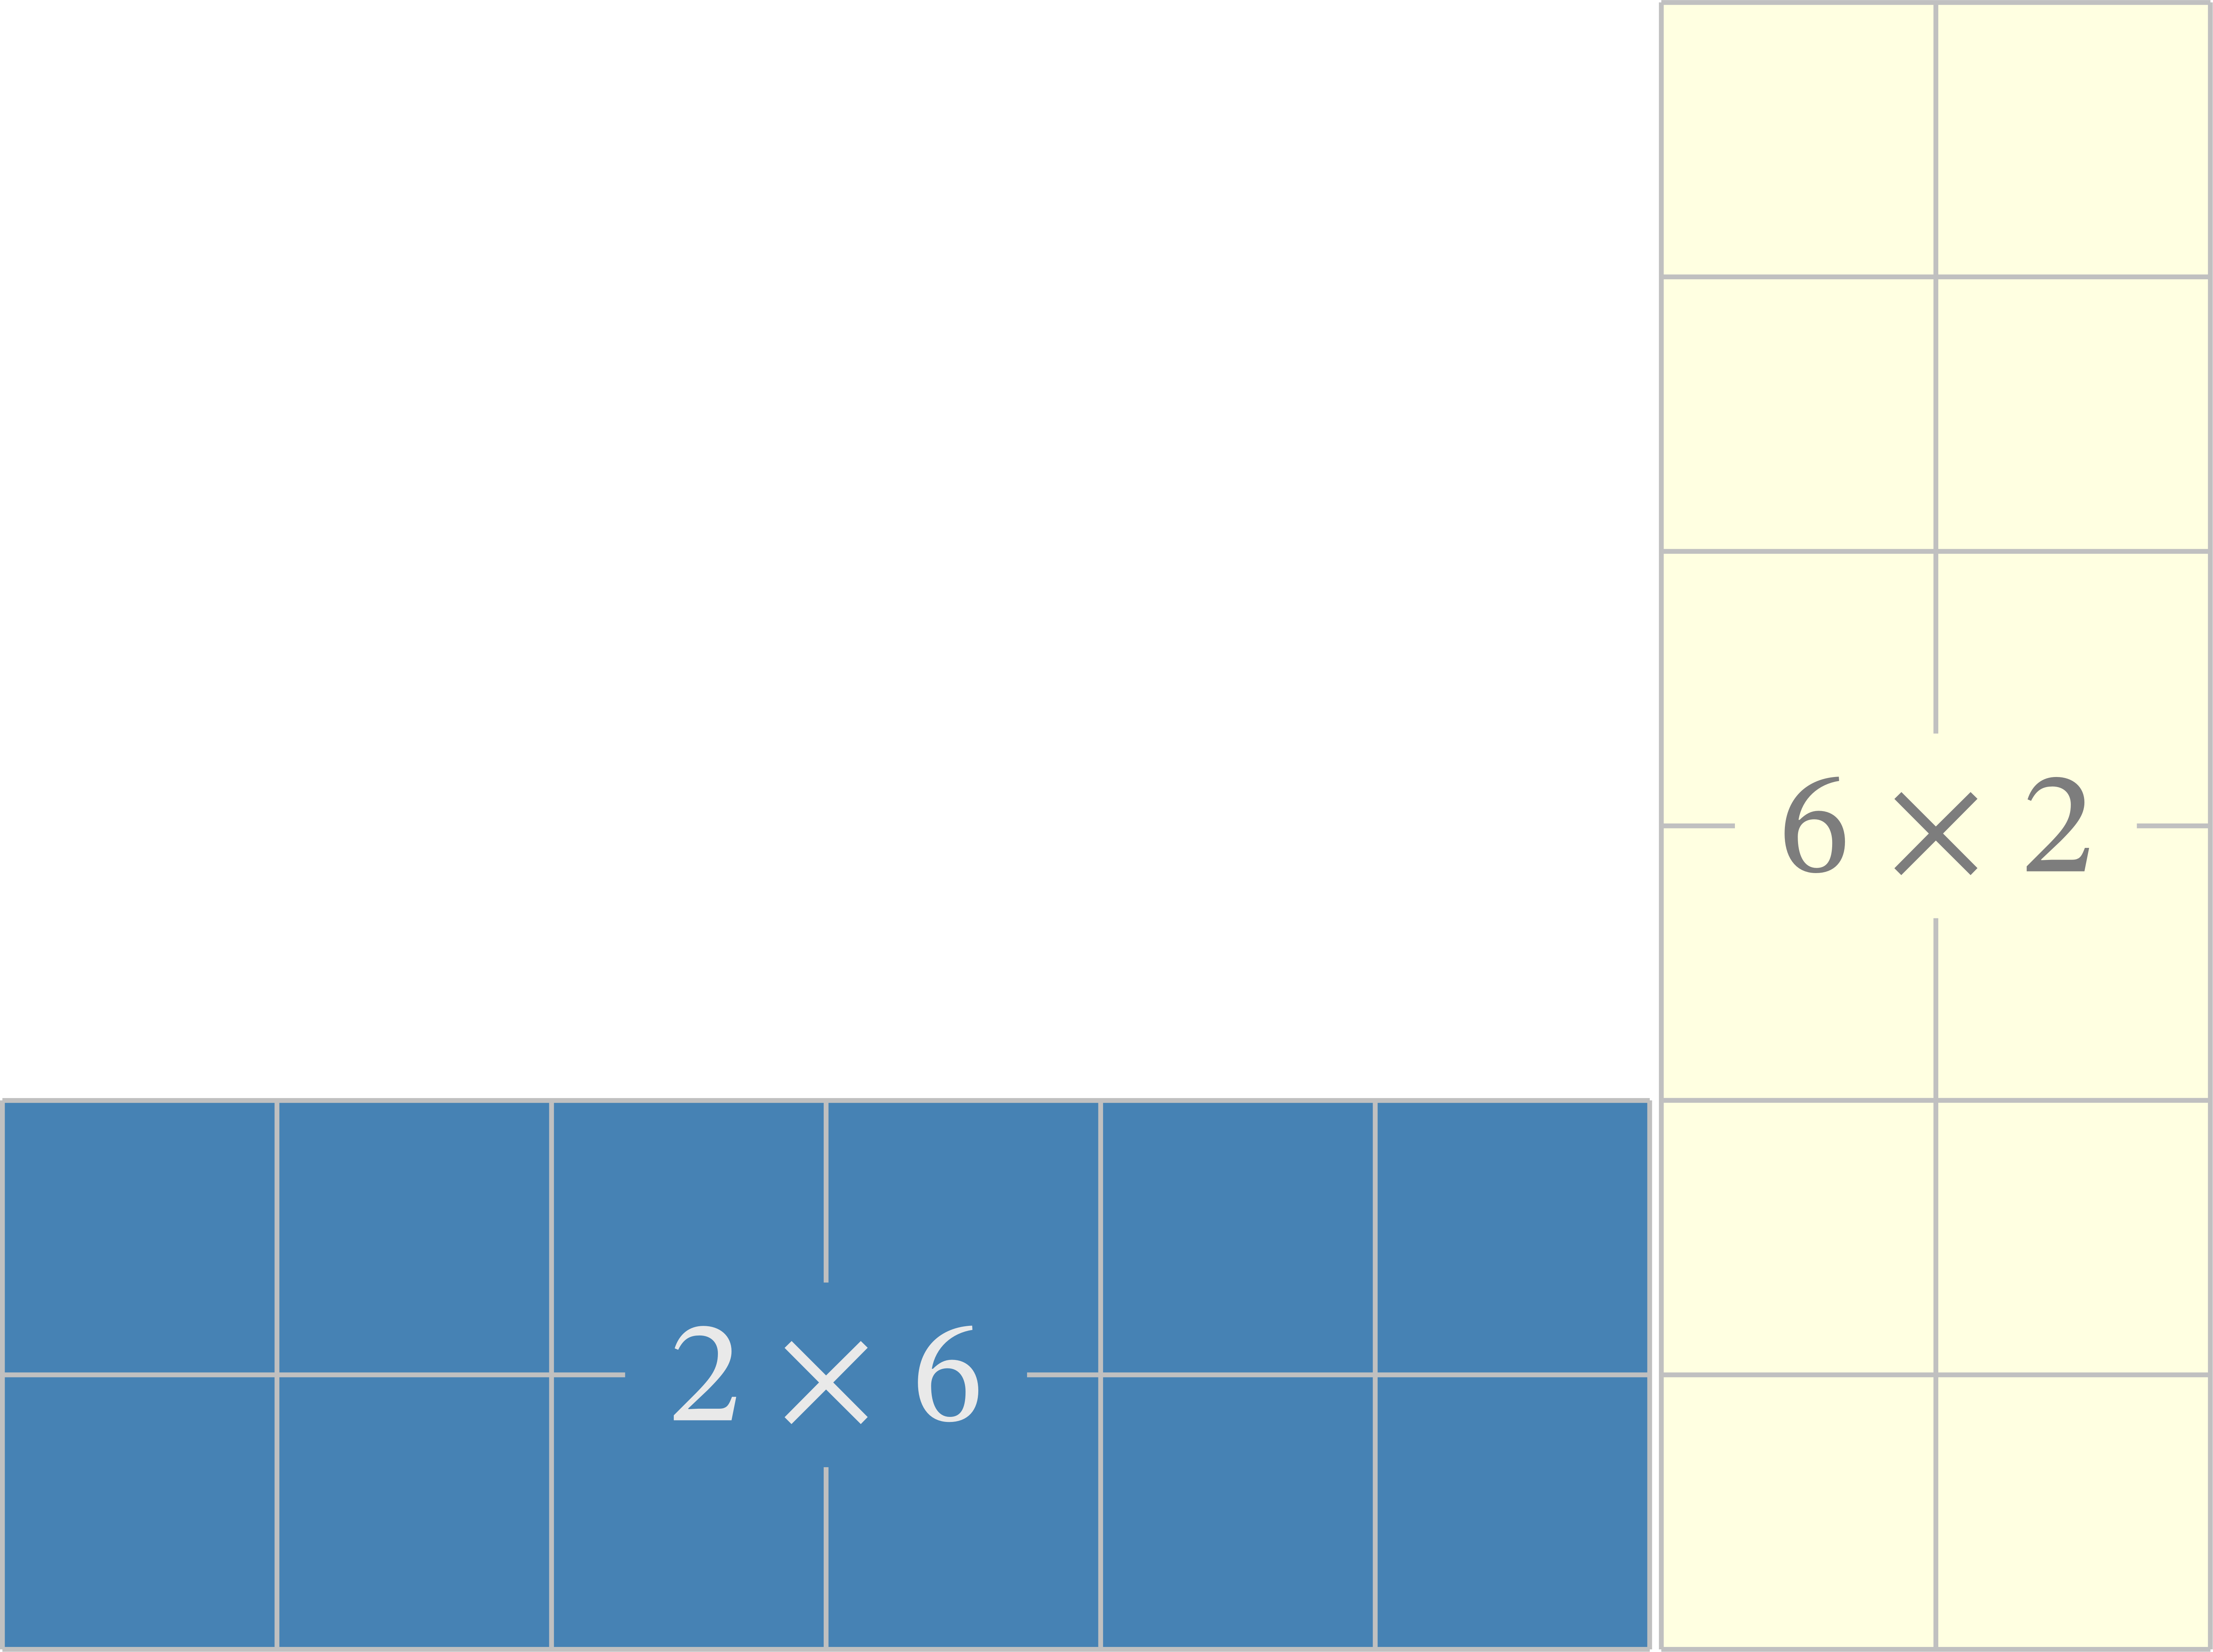
\includegraphics[width=0.7\textwidth,height=\textheight]{images/six-by-two.png}
\caption{Twelve is a composite number. It may be factorized as
\(2 \times 6\), \(4 \times 3\), or as the trivial
\(1 \times 12\).}\label{fig:six-by-two}
}
\end{figure}

\hypertarget{square-numbers}{%
\subsection{Square numbers}\label{square-numbers}}

A square is a special case of a rectangle whose length and width are
equal. When we write \(3 \times 3 = 9\), and we arrange the resulting
nine squares in a rectangle, we get a \emph{square number} of three
squares by three squares. This is why we say that we are \emph{squaring}
a number when we multiply it by itself.

\begin{figure}
\hypertarget{fig:three-square}{%
\centering
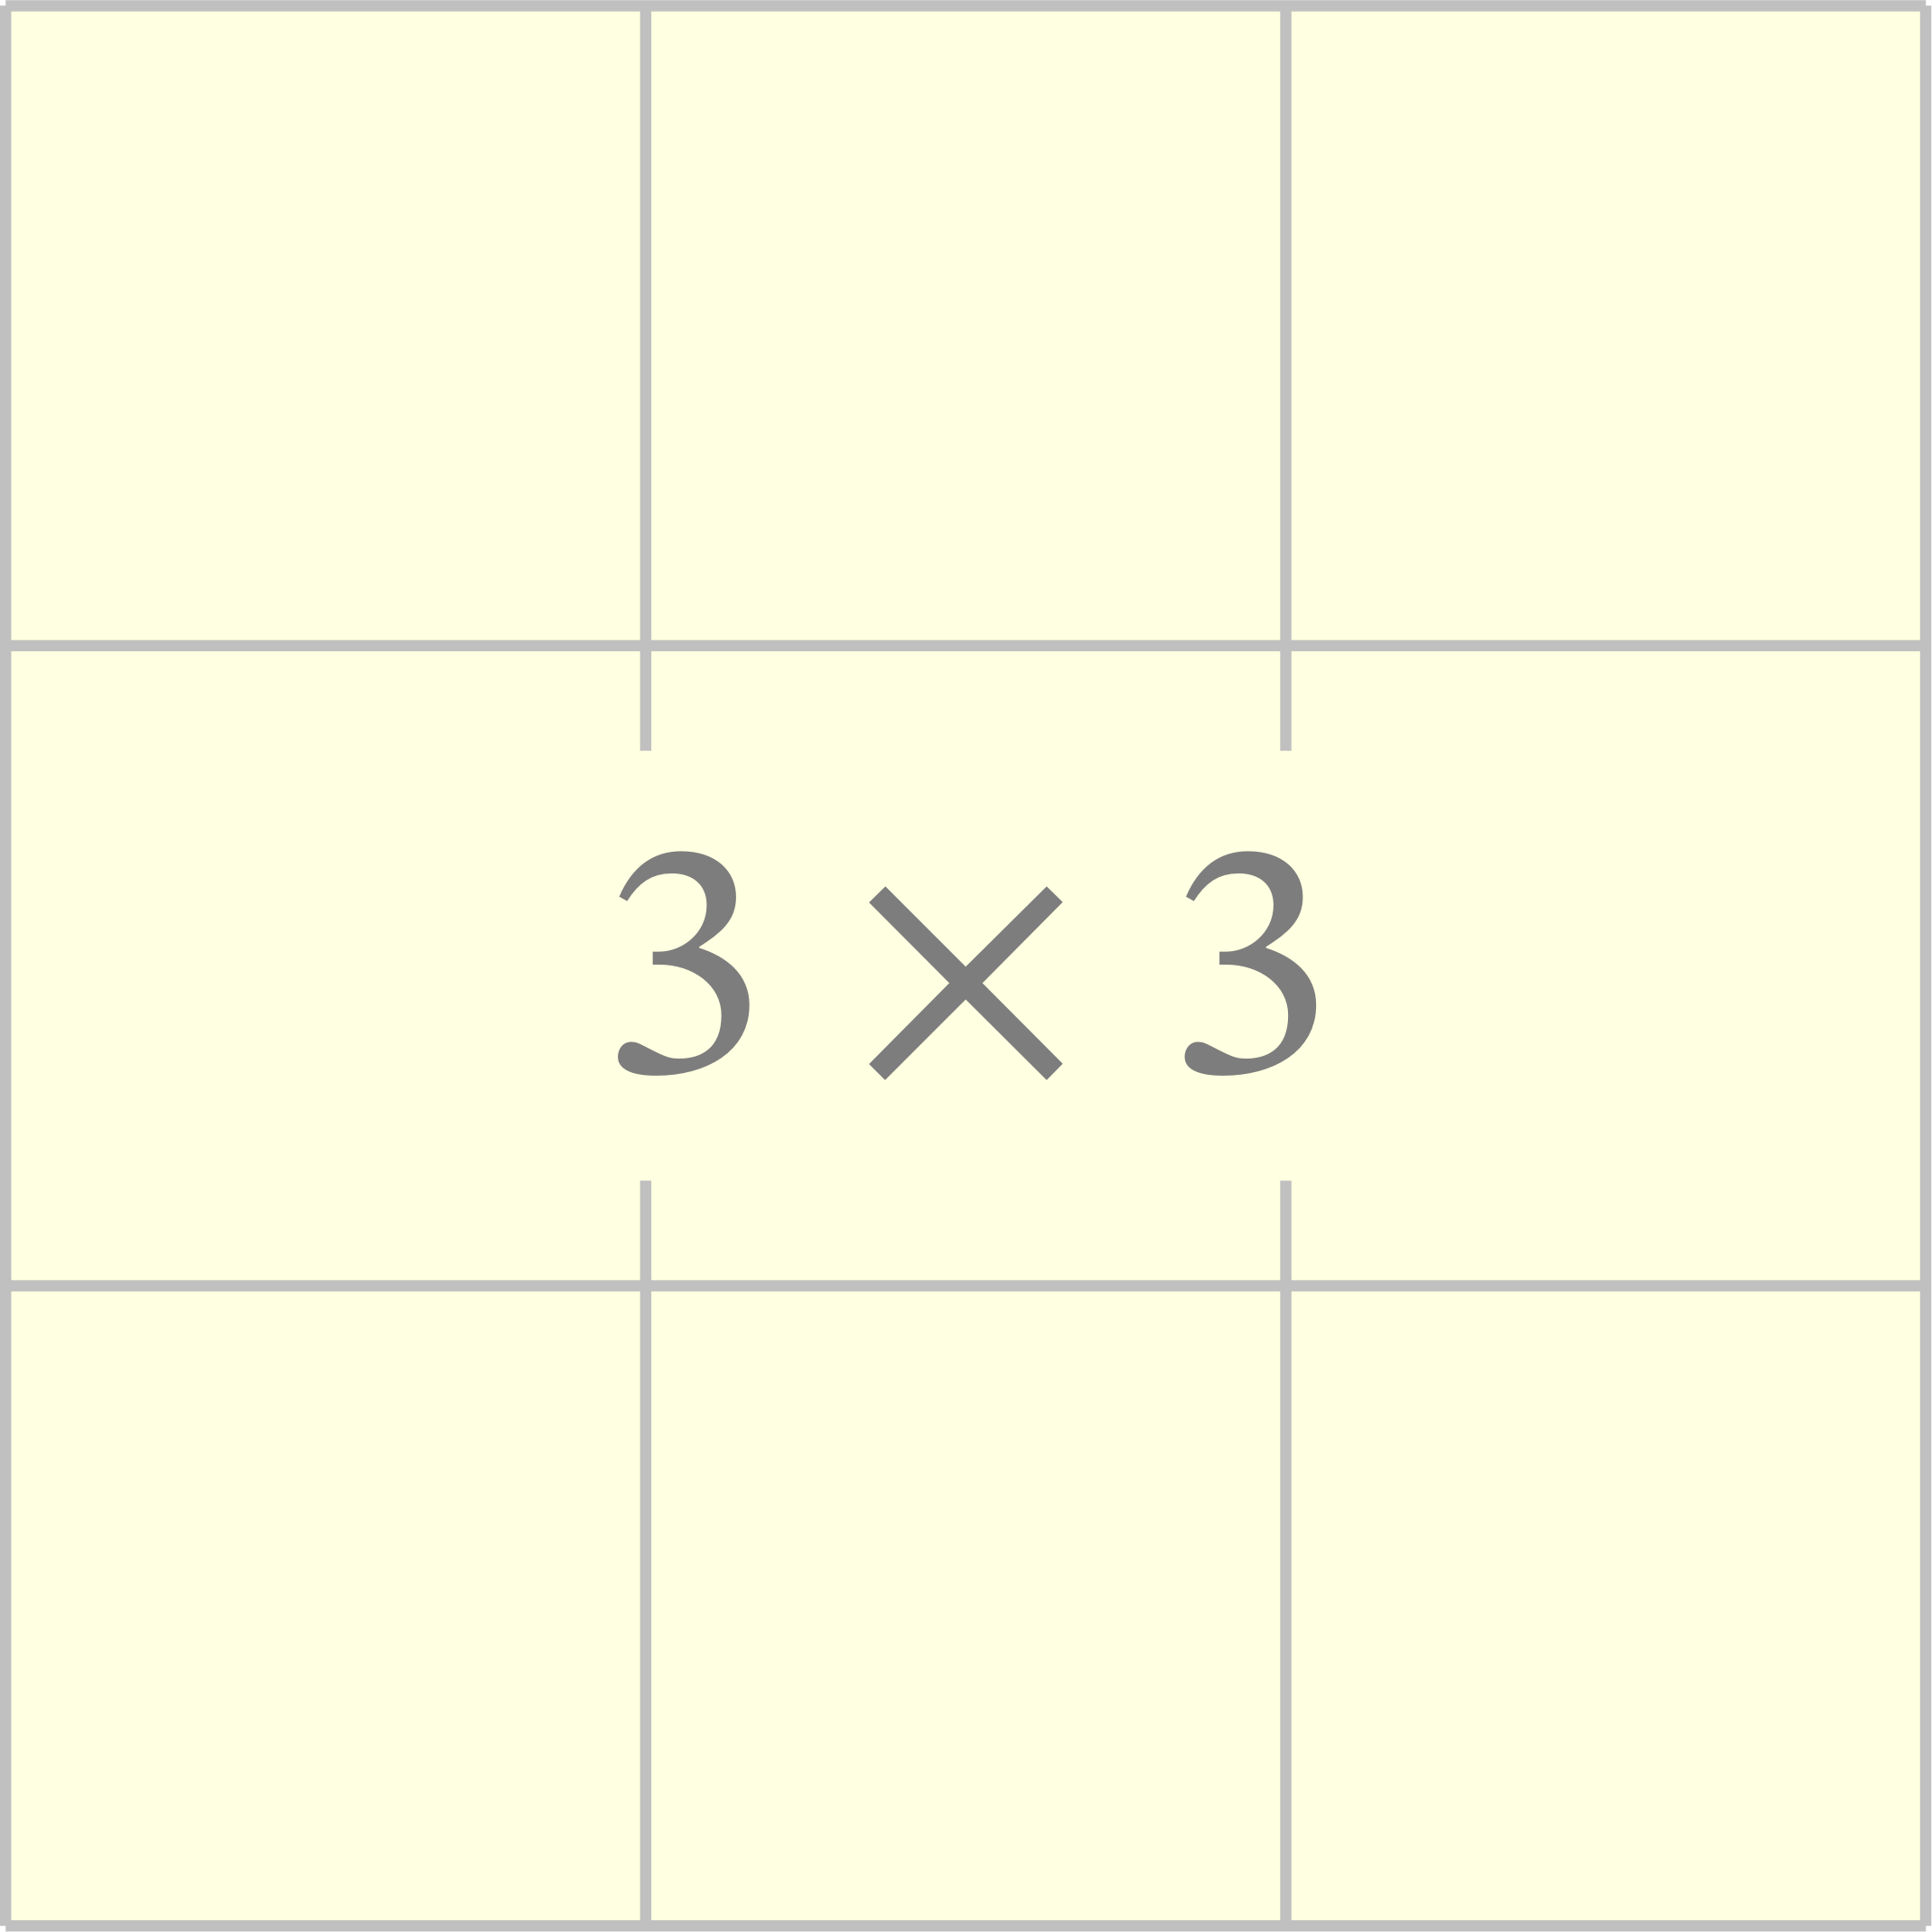
\includegraphics[width=0.2\textwidth,height=\textheight]{images/three-square.png}
\caption{Nine is a square number. Because \(3 \times 3 = 9\), it may be
so portrayed geometrically.}\label{fig:three-square}
}
\end{figure}

One could carry this analogy further and move into three dimensions to
represent a number like \(3 \times 3 \times 3 = 27\) with small cubes
arranged in a large \emph{cube.}\footnote{Try this with toy blocks to
  convince yourself of its truth.} This is why we say we are
\emph{cubing} a number when we multiply it by itself twice.

\hypertarget{prime-numbers}{%
\subsection{Prime numbers}\label{prime-numbers}}

A number which cannot be expressed as the product of two numbers other
than one and itself is called a \emph{prime number}. Prime numbers can
only be arranged in a line, never in a rectangle. Seven is a prime
number as illustrated below.

\begin{figure}
\hypertarget{fig:seven}{%
\centering

\includegraphics[width=0.45\textwidth,height=\textheight]{images/seven.png}
\caption{Seven is a prime number. Its seven icons cannot be re-arranged
in a rectangle.}\label{fig:seven}
}
\end{figure}

Try to rearrange the seven icons into a rectangle to convince yourself
that it is not possible and that seven is prime. Experimenting like this
will help you better understand what testing for primality entails.

Prime numbers are like building blocks that may be used to build larger
numbers by multiplication.

\hypertarget{prime-factorization-is-unique}{%
\subsection{Prime factorization is
unique}\label{prime-factorization-is-unique}}

Let us look at the number \(12\) again, breaking it down this time into
its \emph{prime factors} so: \(12 = 2 \times 2 \times 3\). There are two
instances of the number \(2\) and one instance of the number \(3\).
These numbers cannot be decomposed any further because they are prime.
If we disregard the order of arrangement of these prime factors, i.e.,
we do not distinguish between \(2 \times 2 \times 3\) and
\(2 \times 3 \times 2\) and so on, we may assert that \emph{the prime
factors of a composite number are unique}. This statement is known as
the
\href{https://en.wikipedia.org/wiki/Fundamental_theorem_of_arithmetic}{Fundamental
Theorem of Arithmetic}. It is also sometimes called the Prime
Factorization Theorem.

\hypertarget{symbols-for-multiplication}{%
\subsection{Symbols for
multiplication}\label{symbols-for-multiplication}}

If you are sharp-eyed, you might have come across the multiplication of
two negative numbers by enclosing each of them in parentheses: (). The
same symbols are also used to define associativity and distributivity
later in this blog. We now look at the chequered history of how the
notation for multiplication has changed with time, need, and context.

\hypertarget{times-sign}{%
\subsubsection{Times sign}\label{times-sign}}

The symbol for multiplication that we first learn is the rotated plus
sign ``\(+\)'' that looks like \(\times\). It is called the
``multiplication sign'' and is usually read as ``times'', as we have
already seen. It serves reasonably well even when we outgrow the whole
numbers and move onto fractions.

\hypertarget{parentheses}{%
\subsubsection{Parentheses}\label{parentheses}}

Parentheses, written in pairs as (), have traditionally denoted
\emph{precedence} during evaluation of an expression. Division and
multiplication are evaluated \emph{before} subtraction and addition.
This order may be altered by including terms in parentheses, which are
accorded highest priority during evaluation. So,
\(5 \times 4 + 1 = 20 + 1 = 21\), whereas
\(5 \times (4 + 1) = 5 \times 5 = 25\).

When our discourse embraces negative quantities, in order to avoid
ambiguity, we need something to enclose both the negative sign, \(-\),
and the number to which it applies. The expression \(5 \times -4\) is
ambiguous and therefore never written so when we actually mean
\(5 \times (-4)\). This notation led to two pairs of parentheses
\emph{without any explicit multiplication symbol in between} to denote
the multiplication of the two enclosed numbers thus:
\((5)(-4) = 5 \times (-4) = -20\).

\hypertarget{juxtaposition-without-any-symbol}{%
\subsubsection{Juxtaposition without any
symbol}\label{juxtaposition-without-any-symbol}}

The archetypal symbol for the unknown in algebra is \(x\), which looks a
little too much like the multiplication symbol \(\times\), especially
when handwritten.

To avoid confusion, a convention was adopted that when two
\emph{algebraic variables,} representing unknown quantities, were
written next to each other or \emph{juxtaposed,} it indicated the
multiplication of the two quantities. There is no intervening symbol
between the two variables.

Thus, \(x \times y = (x)(y) = xy\). Note that this convention is for
algebraic variables only. We cannot use this convention with digits
representing numbers because of \emph{place value} in our decimal
system. The number \(45\) does \emph{not} represent the product of \(4\)
and \(5\) but actually means \(40 + 5 = 45\).

\hypertarget{centred-dot}{%
\subsubsection{Centred dot}\label{centred-dot}}

As more exotic objects entered the mathematical collection, yet another
symbol was devised to show (at least one form of) multiplication. The
vertically centred dot \(\cdot\) was used to indicate one of the several
products of \emph{vectors,} which we shall discuss
\protect\hyperlink{dot-or-scalar-product}{later} in this blog. Again,
the dot is not useful in the context of digits because it could be
confused with a decimal point.

So, there is both a rationale and a mathematical context for the
introduction of each symbol for multiplication, according to time, need,
and circumstance.

\hypertarget{asterisk}{%
\subsubsection{Asterisk}\label{asterisk}}

The latter half of the twentieth century saw the introduction of yet
another symbol for multiplication, this time for use in programming
languages. Because the
\href{https://datatracker.ietf.org/doc/html/rfc20}{ASCII character set,}
devised during the era of
\href{https://en.wikipedia.org/wiki/Teleprinter}{teleprinters,} did not
include the symbol \(\times\) for multiplication, another available
symbol had to be chosen for multiplication. The winner was the
\href{https://en.wikipedia.org/wiki/Asterisk}{asterisk}, denoted by *.
Note that even with the symbol *, multiplying \(3\) by \(-4\) still
requires one to type \(3 * (-4)\) to avoid ambiguity.

Repeated multiplication---or
\protect\hyperlink{exponentiation}{exponentiation}---is usually
represented by a double asterisk ** in most computing languages,
although a caret \^{} assumes this function in some languages.

\hypertarget{laws-of-arithmetic}{%
\subsection{Laws of arithmetic}\label{laws-of-arithmetic}}

We now return to the assertion, made at the start of this blog, that
multiplication is a \emph{binary} operation: something that happens
between \emph{two} mathematical objects. You might object that we can
and do multiply three numbers. For example, \(2 \times 3 \times 5 = 30\)
and no one would doubt the veracity of that assertion. Why then is
multiplication classified as a binary operation and how might it be
reconciled with what we know about the multiplication of three or more
numbers?

Early mathematics was eminently practical, concerned with computing
areas and volumes, profit and loss, and so on. In the course of time,
mathematicians started to systematize their body of knowledge by
introducing logic and rigour into their subject. They wanted to move
beyond ad hoc methodology and construct an intellectual edifice that was
stable, durable, and generalizable.

\hypertarget{the-real-numbers-as-a-field}{%
\subsection{The real numbers as a
field}\label{the-real-numbers-as-a-field}}

Some of the most unpleasant experiences of school mathematics are the
sudden and unexpected changes that intrude into the familiar arithmetic
of primary school. Division, fractions, negative numbers, multiplication
by zero, product of two negatives being positive, etc. are a few
examples. When rule upon unanticipated rule is foisted on the young
student, with no rhyme or reason, the student gets overwhelmed and
develops a distaste for mathematics or even a reflex fear of it. This
need not be so.

One way out is a quick but easy introduction to some ideas of abstract
algebra which lay the foundation for all subsequent mathematics. This
way, all the rules are bunched together as unquestioned assumptions.
Then, based on those assumptions, we build a mathematical edifice that
is logical, consistent, and extensible. Mathematics will then be changed
from a mysterious game with unknown rules into a trustworthy friend who
can be depended upon.

The numbers we use every day are drawn from a
\href{https://www.cuemath.com/algebra/sets/}{set} called the
\href{https://mathworld.wolfram.com/RealNumber.html}{real numbers}
denoted by \(\mathbb{R}\). Numbers such as \(0\), \(1\), \(-200\),
\(50004\), \(\frac{1}{2}\), \(-\frac{3}{4}\), \(0.3333\cdots\),
\(-0.5\), \(\sqrt{2}\), \(\pi\), and countless others belong to this
grab bag set.

The set \(\mathbb{R}\) comes bundled with \emph{two} binary operations:
addition, denoted by \(+\), and multiplication denoted by \(\times\) or
by other means as outlined
\protect\hyperlink{symbols-for-multiplication-across-time-and-need}{above}.
One property that makes real numbers so useful is that any addition or
multiplication of real numbers results in another real number---called
\emph{closure}. In addition, the reals also exhibit other familiar
behaviours---with fancy-sounding names---which are tabulated below,
using arbitrary real numbers, \(a, b, c\).

\begin{longtable}[]{@{}
  >{\raggedright\arraybackslash}p{(\columnwidth - 4\tabcolsep) * \real{0.2083}}
  >{\raggedright\arraybackslash}p{(\columnwidth - 4\tabcolsep) * \real{0.3472}}
  >{\raggedright\arraybackslash}p{(\columnwidth - 4\tabcolsep) * \real{0.3611}}@{}}
\caption{Algebraic Properties of \(\mathbb{R}\)\\
}\tabularnewline
\toprule\noalign{}
\begin{minipage}[b]{\linewidth}\raggedright
Property
\end{minipage} & \begin{minipage}[b]{\linewidth}\raggedright
Addition
\end{minipage} & \begin{minipage}[b]{\linewidth}\raggedright
Multiplication
\end{minipage} \\
\midrule\noalign{}
\endfirsthead
\toprule\noalign{}
\begin{minipage}[b]{\linewidth}\raggedright
Property
\end{minipage} & \begin{minipage}[b]{\linewidth}\raggedright
Addition
\end{minipage} & \begin{minipage}[b]{\linewidth}\raggedright
Multiplication
\end{minipage} \\
\midrule\noalign{}
\endhead
\bottomrule\noalign{}
\endlastfoot
Associativity & \((a+b)+c=a+(b+c)\) & \((ab)c = a(bc)\) \\
Commutativity & \(a+b=b+a\) & \(ab=ba\) \\
Identity & \(a+0=a=0+a\) & \(a·1=a=1·a\) \\
Inverse & \(a+(-a)=0=(-a)+a\) & \(aa^{-1}=1=a^{-1}a\) for \(a \ne 0\) \\
\end{longtable}

For the record, formal definitions for the above terms are available on
the Web from reputable sites whose links are listed below:

\begin{enumerate}
\item
  \href{https://mathworld.wolfram.com/Associative.html}{Associativity}.
\item
  \href{https://mathworld.wolfram.com/Commutative.html}{Commutativity}.
\item
  \href{https://en.wikipedia.org/wiki/Distributive_property}{Distributivity}.
  Multiplication is distributive over addition. For completeness, we
  define \[
  \begin{array}{l  l}
  \mbox{Left Distributivity} & a(b+c)=ab+ac\\
  \mbox{Right Distributivity} & (a+b)c=ac+bc\\
  \end{array}
  \] In our case, both conditions hold, and we may simply say that
  \emph{multiplication is distributive over addition for the reals}. A
  mathematical object consisting of a set with two binary operations
  having the above properties is called a
  \href{https://en.wikipedia.org/wiki/Field_(mathematics)}{field}. We
  may refer to the field of real numbers.
\end{enumerate}

\hypertarget{associativity-of-multiplication}{%
\subsection{Associativity of
multiplication}\label{associativity-of-multiplication}}

\emph{Because multiplication is binary, we can only multiply two numbers
at any one time.} If we need to multiply together three or more numbers,
we have to multiply two of them first to get a single product before we
can multiply it with next number, and so on.

The associative law simply states that when we multiply three numbers,
it does not matter which two of the three we multiply first; the result
will always be the same. It is this property that allows us to write
something like \(2 \times 3 \times 5\) or \(abc\) and still make
sense---because it denotes something unique---even though we know that
multiplication is a binary operation.

\hypertarget{the-additive-and-multiplicative-inverses-in-mathbbr}{%
\subsection{\texorpdfstring{The additive and multiplicative inverses in
\(\mathbb{R}\)}{The additive and multiplicative inverses in \textbackslash mathbb\{R\}}}\label{the-additive-and-multiplicative-inverses-in-mathbbr}}

In addition to the three properties of associativity, commutativity, and
distributivity, the real numbers we use every day have two other
properties:

\begin{enumerate}
\item
  \href{}{Additive inverse}: \(a + (-a) = (-a) + a = 0\).
\item
  \href{}{Multiplicative inverse}:
  \(a \times \frac{1}{a} = \frac{1}{a} \times a = 1 \mbox{ for } a \ne 0\).
\end{enumerate}

If you are wondering where subtraction and division have been hiding,
they are hiding in plain sight. Subtracting \(b\) from \(a\) amounts to
adding the additive inverse of \(b\) to \(a\). So, \[
a - b = a + (-b)
\] Likewise, dividing \(a\) by \(b \ne 0\) amounts to multiplying \(a\)
by the multiplicative inverse of \(b\) which equals \(\frac{1}{b}\): \[
a \div b = a \times \frac{1}{b} = \frac{a}{b} \mbox{ for } b \ne 0.
\]

\hypertarget{multiplying-with-zero-always-gives-zero}{%
\subsubsection{Multiplying with zero always gives
zero}\label{multiplying-with-zero-always-gives-zero}}

When an arbitrary number \(a \in \mathbb{R}\) is multiplied by zero, the
product is always zero. To understand why this must be so, let us for
convenience consider a simple but concrete example: \(5 \times 0\). Here
\(5\) is the multiplier and \(0\) the multiplicand. So, we may write: \[
\begin{aligned}
5 \times 0 &= 0 + 0 + 0 + 0 + 0; & \mbox{ multiplication is repeated addition}\\
&= (0 + 0) + (0 + 0) + 0; & \mbox{ addition is a binary operation}\\
&= (0 + 0) + 0; & \mbox{ $0$ is the additive inverse}\\
&= 0. & \mbox{ $0$ is the additive inverse}\\
\end{aligned}
\] We have carefully tiptoed our way to justify each step with one of
the field axioms. And the choice of a whole number made it easy to see
the multiplication as repeated addition. What about \(0 \times 5\)?
Because multiplication is commutative, we may assert that \(0 \times 5\)
is also \(0\), without doing any additional work. I hope you are getting
to see mathematics as treasure hunt with clues and short cuts that lead
to an exciting finale.

\hypertarget{product-of-a-positive-and-a-negative-number}{%
\subsubsection{Product of a positive and a negative
number}\label{product-of-a-positive-and-a-negative-number}}

Negative numbers arose when loans had to be given and taken. They also
find use in describing the depth of an ocean trench as being so much
\emph{below} sea level. Other applications arise naturally with
temperatures below the freezing point or with electric charges of a
negative type, etc.

Consider \(a > 0, b > 0 \in \mathbb{R}\). Knowing that \(a\) is positive
and \((-b)\) is negative, what is the sign of the product \((a)(-b)\)?
To answer this question, let us add \(ab\) to \((a)(-b)\). \[
\begin{aligned}
ab + (a)(-b) &= a(b + (-b)); & \mbox{ distributive law}\\
&= a(0); & \mbox{ $-b$ is the additive inverse of $b$}\\
&=0. & \mbox{ zero multiplied by any number is zero}\\
\end{aligned}
\] Therefore, \(ab + (a)(-b) = 0\) which implies that they are
themselves additive inverses. So, \((a)(-b) = -(ab)\) which is a
negative number. Conversely, a negative number may be split into the
product of a positive number and a negative number.

This explanation might seem contrived but it provides guardrails against
falling off when future mathematical objects are encountered. And it is
a whole lot more satisfying than hand-waving or saying ``Just take it on
faith.''

\hypertarget{why-is-the-product-of-two-negative-numbers-positive}{%
\subsubsection{Why is the product of two negative numbers
positive?}\label{why-is-the-product-of-two-negative-numbers-positive}}

If you have no qualms accepting negative numbers, you might still be
confounded by what we could mean by multiplying two negative numbers.
The answer, which might startle you, is that \emph{the product of two
negative numbers is a positive number.}

Let us use the field axioms to navigate our way through this result as
well. Let \(a > 0, b > 0 \in \mathbb{R}\). Then, both \((-a)\) and
\((-b)\) are negative. Note that \(ab\) is positive and its additive
inverse is \(-(ab) = (-a)(b) = (a)(-b)\) which is negative from our
previous result.

The scheme we have followed so far is to add something to the object of
interest and use the axioms to prove that the sum is zero. The result we
are after will then pop out. Let us apply that method again. \[
\begin{aligned}
-(ab) + (-a)(-b) &= (a)(-b) + (-a)(-b); & \mbox{ result from previous section}\\
&= (a + (-a))(-b) & \mbox{ distributive law}\\
&= (0)(-b) & \mbox{ additive inverse}\\
&= 0. & \mbox{ zero mutiplied by anything is zero}\\
\end{aligned}
\] The upshot is that we have \(-(ab) + (-a)(-b) = 0\) which means that
they are additive inverses. Since the additive inverse of \(-(ab)\) is
\(ab\), we conclude that \((-a)(-b) = ab\) implying that the product of
two negative numbers is a positive number. With the axioms to guide us,
we can move with the sure-footedness of a mountain goat as we scale the
heights and depths of each proof.

I have dealt with the arithmetic of fractions and negative numbers in my
freely downloadable chapter ``Arithmetic Revisited'' from
\href{https://swanlotus.netlify.app/sas-manuscript/SAS-partial.pdf}{\emph{Secrets
of Academic Success}}. I urge you to read it if you feel the need.

\hypertarget{exponentiation}{%
\section{Exponentiation}\label{exponentiation}}

Just as multiplication with whole numbers is repeated addition,
exponentiation is repeated multiplication. A new notation is used to
indicate repeated multiplication. We denote it by a \emph{superscript}
indicating how many times the number is multiplied:
\(5 \times 5 \times 5 = 5^{3}\), and so on. The number \(5\) is called
the \emph{base} and \(3\) the \emph{exponent}. We call the number
\(5^{3}\) as ``five cubed'' for reasons already explained, or as ``five
(raised) to the (power of) three''.

What is the exponent in the number \(5?\) The base is \(5\) but the
exponent is \emph{implicit} or understood but not written. If we take
\(5 = 5^{1}\), the
\(5 \times 5 \times 5 = 5^{1} \times 5^{1} \times 5^{1} = 5^{3}\). When
we multiply numbers with the same base, we can simply add the exponents.
And this fact underlies a very powerful computational
device---logarithms.

\hypertarget{logarithms-multiplying-by-adding}{%
\section{Logarithms: multiplying by
adding}\label{logarithms-multiplying-by-adding}}

We may reduce multiplication to addition if we focused on the exponent
of a common base. This is exactly what was done by an eccentric Scottish
laird called
\href{http://www-history.mcs.st-andrews.ac.uk/Biographies/Napier.html}{John
Napier} whose labours have made all our lives much less tedious. The
books of logarithmic tables, affectionately called ``log books'' when I
was at school, along with the \href{http://sliderulemuseum.com/}{slide
rule} were the mainstay of physicists and engineers before the advent of
the electronic calculator in the mid-1970s. And they all relied on
Napier's scheme of reducing multiplication to addition.

Multiplying by adding is simple. Suppose we want to multiply \(2\) by
\(3\). We follow this algorithm:

\begin{enumerate}
\item
  Express the number \(2\) as a power of \(10\):
  \(2 \approx 10^{0.30103}\).
\item
  Express the number \(3\) as a power of \(10\):
  \(3 \approx 10^{0.47712}\).
\item
  Add the two powers or exponents: \(0.30103 + 0.47712 = 0.77815\).
\item
  Find out what number equals \(10^{0.77815}\). In our case,
  \(10^{0.77815} \approx 5.99998\).
\end{enumerate}

``Aha!'' you might say. ``But the answer is not exactly \(6\) which is
the correct answer.'' You are right. With logarithms and the limited
number of digits of precision, we can at best obtain a very good
approximation to a computation.

If you had to compute \(23.589 \times 459.1213\) what would you do? You
would run to a calculator and punch in the digits to get \(10830.212\)
with very little effort today. But if you lived in a period without
electronic calculators, you would be very glad that logarithms existed,
and you would happy to chirp out the answer as \(10830.213\) thanks to
Napier.

\hypertarget{square-roots}{%
\section{Square roots}\label{square-roots}}

Taking a square root is a form of \emph{exponentiation}. If I gave you a
number like \(9\) and asked you to find a number such that when it was
\emph{added} to itself, you would get \(9\), you would almost
instinctively divide \(9\) by \(2\) to give me \(4.5\) and indeed
\(4.5 + 4.5 = 9\).

If instead, I asked you to find that number, which when
\emph{multiplied} by itself gives \(9\), how would you go about solving
it? We know that in this case, the answer is \(3\) because
\(3 \times 3 = 9\). To approach it systematically, we need a symbol for
the operation, which when performed on \(9\) gives us \(3\). For
historical reasons it was called \emph{taking the square root} and the
symbol \(\surd\) is a stylized letter ``r'' for ``radix'' meaning
``root'' in Latin. So, we write \(\sqrt{9} = 3\).

But is that the whole story? Recall that the product of two negative
numbers is positive. So, \((-3)(-3) = 9\) as well. So, which is the
``true'' or ``correct'' square root? By convention, we associate the
positive square root with the symbol \(\surd\). So, without any
ambiguity, \(\sqrt{9} = 3\) and \(-\sqrt{9} = -3\).

\hypertarget{complex-numbers}{%
\section{Complex numbers}\label{complex-numbers}}

Talking about square roots and negative numbers, can we ever take the
square root of a negative number? Do such numbers exist? If so, where?
And are they useful?

The squares of real numbers give rise to only two possibilities. The
square of zero is zero. The square of any non-zero real number, whether
positive or negative, is always positive, as we have just seen. So, the
possibility of a negative number being the square of a real number does
not ever arise.

But we do encounter a different situation when solving an algebraic
equation like \(x^{2} + 4 = 0\). When such equations were first
encountered, mathematicians simply said that they had \emph{no
solutions.} This is true even when you initially encounter them at
school today. \emph{This equation has no solution in the field of real
numbers.}

In the course of time, these pesky numbers---whose square is a negative
number---kept popping up insistently in unlikely places. They were then
reluctantly assigned mathematical existence with the somewhat pejorative
term \emph{imaginary numbers.} They were after all \emph{not real
numbers!}

In the course of time, a sandwich number was invented which was composed
of the sum of a real number and an imaginary number. This number was
called a \emph{complex number.} It is the first of several mathematical
objects we will encounter in this blog that are different from the real
numbers of everyday life.

The number \(5 + 2i\) is a complex number. Its real part is, of course,
\(5\) and its imaginary part is \(2i\).

The symbol \(i\) is called the \emph{imaginary unit} and is the solution
of the equation \(i^2 + 1 = 0\).\footnote{Because \(i\) is often
  associated with current, electrical engineers often use the symbol
  \(j\) instead.} Note that this definition of \(i\) is not unique
because there are two solutions, one positive and one negative. By
convention, we take \(+i = i\) to be one root and \(-i\) to be the
other. The notion of positive and negative roots does not have the same
significance it did with the real numbers, but we should be aware of the
ambiguity in the definition.

\hypertarget{multiplication-of-complex-numbers}{%
\section{Multiplication of complex
numbers}\label{multiplication-of-complex-numbers}}

When we multiply complex numbers, we are really performing
multiplication on \emph{two pairs} of real numbers with the imaginary
unit sandwiched in between. Because of the property \(i^2 = -1\), the
rules of multiplication with terms involving \(i\) must be modified to
honour this equation. Let us see how, with a step-by-step example: \[
\begin{aligned}
(2 + 3i)(4 - 5i) & = 2(4) + 2(-5i)\\
& \quad + (3i)(4) + (3i)(-5i)\\
& = 8 - 10i + 12i + (-15)(i^2)\\
& = 8 + 2i + (-15)(-1)\\
& = 23 + 2i.
\end{aligned}
\] Note that we use \(i^2 = -1\) and group like terms, but otherwise
proceed as normal. If we were to generalize this to a pair of complex
numbers, we get \[(a + bi)(c + di) = (ac - bd) + (ad + bc)i.\]

\hypertarget{polar-form-of-complex-numbers}{%
\subsection{Polar form of complex
numbers}\label{polar-form-of-complex-numbers}}

\(re^{i\theta} = r(\cos\theta + i\sin\theta)\)

\hypertarget{consistency-between-real-and-complex-multiplication}{%
\subsection{Consistency between real and complex
multiplication}\label{consistency-between-real-and-complex-multiplication}}

What happens if we used the rule for complex multiplication above but
set the imaginary parts to zero so that complex multiplication reverts
to the multiplication of two real numbers? Do we get consistent results?
Let us try it by substituting \(b = d = 0\) in the above case. We then
have: \[
\begin{aligned}
(a + 0i)(c + 0i) & = [ac - (0)(0)] + [a(0) + (0)c]i\\
& = ac.
\end{aligned}
\] It is a great relief that the result is as expected. The
multiplication of two complex numbers gives us the same result as the
earlier definition for multiplication of two real numbers when we set to
zero the imaginary parts of the two complex numbers. The definitions of
real and complex multiplication are therefore consistent.

It is a primary requirement in mathematics that when we extend the
definition of an operation on a simpler object to encompass a more
complicated mathematical object, the new definition should revert to the
accepted definition for the simpler object when the complicated object
reverts into the simpler object. This is the point about consistency
that I made at the start of this blog.

\hypertarget{complex-numbers-as-ordered-pairs}{%
\subsection{Complex numbers as ordered
pairs}\label{complex-numbers-as-ordered-pairs}}

Arithmetic operations on complex numbers result only in complex numbers
and do not give rise to new types of numbers. And all complex numbers
consist of two parts: a real part and an imaginary part.

Hence, if we develop a new notation for this two-part number for
purposes of arithmetic, we may dispense altogether with the symbol
\(i\), which after all, seems somewhat out of place in a numerical
context.

The simplest notation is to represent complex numbers as
\href{http://www.mathsisfun.com/definitions/ordered-pair.html}{\emph{ordered
pairs}} of real numbers with the convention that the first number is the
real part and the second number is the imaginary part. Once we have done
this, we need to re-define all the arithmetic operations for these
ordered pairs.

We may thus use the ordered pair \((a, b)\) to denote the complex number
\(a + bi\) and likewise, \((c, d)\) for the complex number \(c + di\).

Drawing upon our previous results, we may then \emph{define}
multiplication for this ordered pair as being \[
(a, b)\cdot(c, d) = (ac - bd, ad + bc).
\] Note that order matters here: the first number of the ordered pair is
the real part of the complex number and the second is the imaginary
part. We cannot swap them willy nilly.

\hypertarget{vectors}{%
\section{Vectors}\label{vectors}}

Ordered pairs lead rather neatly to the idea of
\href{http://en.wikipedia.org/wiki/Euclidean_vector}{\emph{vectors.}}\footnote{Properly
  called Euclidean vectors in our context.} Indeed, there is more than a
passing resemblance between complex numbers and two-dimensional vectors.

Both may be represented by ordered pairs of real numbers and the rules
for addition and subtraction of these ordered pairs are identical.
Moreover, they may both be represented as points on a
\href{http://en.wikipedia.org/wiki/Cartesian_coordinate_system}{Cartesian
plane.}

Vectors are the second new mathematical object, after complex numbers,
that we are meeting in this blog.

{[}caption id=``attachment\_87'' align=``alignleft'' width=``130''{]}
Two vectors shown as directed line segments.{[}/caption{]}

A \emph{vector} is traditionally defined as a quantity having two
attributes: \emph{magnitude} and \emph{direction.} A simple everyday
example is the wind which has both a speed and direction, and may
therefore be represented by a vector. Indeed, if you have already
encountered vectors, you might think of them exclusively as
\emph{directed line segments} or lines of specific lengths with arrow
tips as shown.

\hypertarget{addition-and-subtraction-of-vectors-geometric-viewpoint}{%
\subsection{Addition and subtraction of vectors: geometric
viewpoint}\label{addition-and-subtraction-of-vectors-geometric-viewpoint}}

How do we add and subtract these geometric entities, let alone multiply
and divide them? If you have done physics at high school, you will know
that we use something called the \emph{parallelogram law.}

We draw a pair of two-dimensional vectors so that both originate from
the same point. We then complete the parallelogram formed by these two
vectors by drawing in the other two sides. The \emph{sum} of the two
vectors, or their \emph{resultant,} is the diagonal of the parallelogram
that starts at the same origin as the two vectors. This is something
best grasped from a picture:

{[}caption id=``attachment\_88'' align=``aligncenter'' width=``351''{]}
The parallelogram law for the addition of two vectors.{[}/caption{]}

The origin of the Cartesian plane is labelled \(O\). We have three named
vectors and three ordered pairs indicate the positions of their arrow
tips:

\begin{enumerate}
\tightlist
\item
  \(\mathbf{u}\) : the vector from \(O\) to the point \((8, 4);\)
\item
  \(\mathbf{v}\) : the vector from \(O\) to the point \((2, 6);\) and
\item
  \(\mathbf{w}\) : the vector from \(O\) to the point \((10, 10)\).
\end{enumerate}

The dotted grey lines indicate the two sides of the parallelogram that
we draw to close the figure. The vector \(\mathbf{w}\) is the diagonal
that represents the sum of \(\mathbf{u}\) and \(\mathbf{v}\). This sum
is written as \[
\mathbf{u} + \mathbf{v} = \mathbf{w}
\] If you look at the illustration carefully, you would note that if we
added the first co-ordinate of \(\mathbf{u}\) and the first co-ordinate
of \(\mathbf{v}\) we get the first co-ordinate of \(\mathbf{w}\). And
likewise for the second co-ordinate.

So, we may represent the addition of \(\mathbf{u}\) and \(\mathbf{v}\)
as \[
(8, 4) + (2, 6) = ((8+2), (4+6)) = (10, 10)
\] This is no accident. Nor is it a special case. It works for all
parallelograms.\footnote{I leave it to you to convince yourself of this.
  (Hint: use graph paper, draw the co-ordinate axes, and use algebraic
  variables for the co-ordinates of \(\mathbf{u}\), \(\mathbf{v}\), and
  \(\mathbf{w}\).)}

The parallelogram law is a geometric statement of what happens when we
add two ordered pairs the way we would two complex numbers: \[
(a, b) + (c, d) = (a+c, b+d)
\] We may therefore dispense with line segments and arrow tips and
abstract vectors as ordered pairs even as we rescued complex numbers
from explicit association with \(i\).

\hypertarget{addition-and-subtraction-of-vectors-algebraic-viewpoint}{%
\subsection{Addition and subtraction of vectors: algebraic
viewpoint}\label{addition-and-subtraction-of-vectors-algebraic-viewpoint}}

We may identify two-dimensional vectors \emph{uniquely} by an ordered
pair representing their co-ordinates on the Cartesian plane. This is the
algebraic viewpoint. It is less cumbersome and more powerful as we have
already seen from the addition of two vectors.

Subtraction is equally simple. There is no need to reverse vectors and
draw another parallelogram. We simply say: \[
(8, 4) - (2, 6) = (6, -2)
\] It really cannot get any simpler than that! :-)

\hypertarget{vectors-as-algebraic-entities}{%
\subsection{Vectors as algebraic
entities}\label{vectors-as-algebraic-entities}}

We have just seen that two-dimensional vectors may be represented by
ordered pairs on the Cartesian plane. This representation might be
extrapolated to include vectors of dimensions greater than two.
Obviously, we would then be moving from ordered pairs to ordered
triples, etc.\footnote{An ordered triple, for example, would live in our
  familiar three-dimensional space.}

To generalize, we may think of vectors as a list of ``numbers in a
teabag'' where their order matters. Formally, an \(n\)-dimensional
vector is an \emph{ordered list} of \(n\) numbers written within
enclosing parentheses or brackets and treated as a \emph{single entity.}
This is also called an
\href{http://en.wikipedia.org/wiki/Tuple}{\emph{ordered n-tuple.}} Each
individual number is called a \emph{component} of the vector.

The components of a vector may be written within parentheses or
brackets. They may be arranged vertically as a \emph{column vector} of a
single column and \(n\) rows or horizontally as a \emph{row vector} of a
single row and \(n\) columns. A column vector may be \emph{transposed}
into a row vector. Transposition is indicated by the superscript \(T\).
For example, with \(n = 4\) \[
\begin{aligned}
\begin{bmatrix}a\\b\\c\\d\\\end{bmatrix}^{T} & = \begin{bmatrix}a&b&c&d\\\end{bmatrix}\\
\begin{bmatrix}a&b&c&d\\\end{bmatrix}^{T} & = \begin{bmatrix}a\\b\\c\\d\\\end{bmatrix}\\
\end{aligned}
\] Note that there are no commas separating the elements of a row vector
unlike in ordered pairs. Also, we could just as well have used
parentheses as brackets.

It is conventional to assume that an arbitrary vector is a column
vector. Row vectors are then the transposes of the column vectors. This
is the convention we will follow.

\hypertarget{row-column-nomenclature}{%
\subsection{Row-column nomenclature}\label{row-column-nomenclature}}

The size of a vector is denoted by writing down the number of rows
followed by a \(\times\) sign followed by the number of columns. Thus a
column vector with four rows is a \emph{\(4 \times 1\) column vector}
while a row vector with four columns is a \emph{\(1 \times 4\) row
vector.}

By definition, a vector must have at least one dimension equal to \(1\).
When \emph{both} dimensions are equal to one, the vector degenerates
into a single component which, in the context of vectors, is called a
\href{http://en.wikipedia.org/wiki/Scalar_\%28mathematics\%29}{\emph{scalar}}
to distinguish it from a vector.

\hypertarget{addition-and-subtraction-of-vectors}{%
\subsection{Addition and subtraction of
vectors}\label{addition-and-subtraction-of-vectors}}

Addition and subtraction for the ordered n-tuples representing two
vectors may be defined as the addition or subtraction of their
\emph{respective components.}

Just to free ourselves from geometrical thinking about vectors, let us
add two \emph{four-dimensional} vectors whose components are given by
algebraic variables representing real numbers. \[
\begin{bmatrix}a\\b\\c\\d\\\end{bmatrix} + \begin{bmatrix}p\\q\\r\\s\\\end{bmatrix} = \begin{bmatrix}a+p\\b+q\\c+r\\d+s\\\end{bmatrix}
\]

Subtraction is equally ``commonsensical'': \[
\begin{bmatrix}a\\b\\c\\d\\\end{bmatrix} - \begin{bmatrix}p\\q\\r\\s\\\end{bmatrix} = \begin{bmatrix}a-p\\b-q\\c-r\\d-s\\\end{bmatrix}
\]

These vector sums and differences would be difficult to visualize
geometrically, but they are trivially routine algebraically.

\hypertarget{multiplication-of-vectors}{%
\section{Multiplication of vectors}\label{multiplication-of-vectors}}

It is easy to think of the addition or subtraction of vectors, say in
the context of ``wind speed'' and ``air speed'' of an aircraft. But what
does the multiplication of vectors consist of and what meaning could we
extract from the operation?

Vector multiplication is a strange, many-headed beast. It is important
to know what it is and what it is not. Here is a quick run down:

\begin{enumerate}
\def\labelenumi{\arabic{enumi}.}
\item
  Vector multiplication is different from real multiplication.
\item
  Vector multiplication is different from complex multiplication.
\item
  There are several varieties of vector multiplication, some of which
  give us scalars, others vectors, and still others matrices:\footnote{Ignore
    any unfamiliar terms for now.}

  \begin{enumerate}
  \def\labelenumii{(\alph{enumii})}
  \tightlist
  \item
    multiplication of a vector by a scalar to yield a vector
  \item
    \href{http://mathworld.wolfram.com/DotProduct.html}{dot product} or
    scalar product or inner product of two vectors to yield a scalar
  \item
    \href{http://mathworld.wolfram.com/CrossProduct.html}{cross product}
    of two vectors to yield a third vector orthogonal to the other two
  \item
    \href{http://en.wikipedia.org/wiki/Tensor_product}{tensor product}
    or \href{http://en.wikipedia.org/wiki/Outer_product}{outer product}
    of two vectors to yield a matrix
  \end{enumerate}
\end{enumerate}

\begin{enumerate}
\def\labelenumi{\arabic{enumi}.}
\setcounter{enumi}{3}
\item
  Each variety of vector product was devised as an operation because it
  is useful and has a ready meaning in a particular context.
\item
  When it comes to multiplication, vectors reveal their nature as a
  class of mathematical object quite different from real or complex
  numbers.
\end{enumerate}

Let us consider each type of multiplication in turn.

\hypertarget{multiplication-by-a-scalar}{%
\section{Multiplication by a scalar}\label{multiplication-by-a-scalar}}

Multiplication of a vector by a scalar is the easiest to understand. In
this operation, we see the original arithmetic definition of real
multiplication at play. We are magnifying or diminishing the magnitude
of the vector by multiplying it with a scalar, while the direction of
the vector is either reversed or remains unchanged.

If we have a vector \(\mathbf{u}\) and we multiply it by a scalar \(k\)
the result is the vector \(k\mathbf{u}\). This may be easily visualized
geometrically. If we associate \(\mathbf{u}\) with an arbitrary
four-dimensional column vector, we may write \[
\mathbf{u} = \begin{bmatrix}a\\b\\c\\d\\\end{bmatrix}
\]

Multiplication of \(\mathbf{u}\) by a real scalar \(k\) gives us \[
k\mathbf{u} = k\begin{bmatrix}a\\b\\c\\d\\\end{bmatrix} = \begin{bmatrix}ka\\kb\\kc\\kd\\\end{bmatrix}
\]

When we multiply a vector by a scalar \(k\), each component of the
vector is individually multiplied by \(k\). The magnitude of the
resulting vector takes on a different meanings depending on the value
and sign of \(k\):

\begin{enumerate}
\item
  \(k = 1\): the vector is unchanged in magnitude and direction.
\item
  \(k = -1\): the vector is unchanged in magnitude but reversed in
  direction.
\item
  \(k < -1\): the vector is enlarged in magnitude and reversed in
  direction.
\item
  \(k > 1\): the vector is enlarged in magnitude and unchanged in
  direction.
\item
  \(-1 < k < 0\): the vector is diminished in magnitude and reversed in
  direction.
\item
  \(0 < k < 1\): the vector is diminished in magnitude and unchanged in
  direction.
\item
  \(k = 0\): the vector has zero magnitude and its direction is
  undefined.
\end{enumerate}

While this might seem quite a mouthful, it is really quite simple:

\begin{itemize}
\tightlist
\item
  a negative \(k\) reverses the direction;
\item
  a positive \(k\) keeps the direction unchanged;
\item
  value of \(k\) that lies between \(-1\) and \(0\) or between \(0\) and
  \(1\) diminishes the magnitude; and
\item
  a value of \(k\) less than \(-1\) or greater than \(+1\) increases the
  magnitude of the vector.
\end{itemize}

The special cases pertaining to \(k = \pm 1\) and \(k = 0\) underscore
the paramount importance of \(0\) and \(1\) in the whole of mathematics.
They are keystone numbers.

Did you pick up the fact that after uncoupling geometry and vectors, we
finally resorted to geometry when talking about the meaning of scalar
multiplication? This dual viewpoint runs through much of mathematical
thinking.

Scalar division of vectors by \(k\) is really multiplication by
\(\frac{1}{k}\) and is therefore not considered separately.

If we view scalar multiplication as a black box, it takes in one n-tuple
and gives out another n-tuple. Like the merchant in \emph{Aladdin and
the Wonderful Lamp,} we are simply exchanging old vectors for new. There
is no difference in \emph{kind} between the input and output
mathematical objects.

\hypertarget{the-zero-vector-is-not-the-number-zero}{%
\subsection{The zero vector is not the number
zero}\label{the-zero-vector-is-not-the-number-zero}}

Distinguish carefully between the \emph{real number \(0\)} and the
\emph{n-dimensional zero vector} which results from scalar
multiplication with \(k = 0\). The latter is an n-tuple of zeros and
does \emph{not} equal the real number zero. For example, with \(n = 4\),
the zero vector is: \[
\begin{bmatrix}0\\0\\0\\0\\\end{bmatrix} \neq 0
\]

As and when new mathematical objects are invented (or discovered?) new
definitions for the equivalents of zero and one for these new objects
may also be necessary. The \(n\)-dimensional zero vector is unique as
shown above. But there is no unique n-dimensional unit vector
corresponding to the number \(1\).

We now turn to other varieties of multiplication that may be applied to
vectors.

\hypertarget{dot-or-scalar-product}{%
\section{Dot or scalar product}\label{dot-or-scalar-product}}

The centred dot \(\cdot\) as a symbol for multiplication makes its
appearance here. The first departure from conventional multiplication
was with complex numbers. The
\href{http://en.wikipedia.org/wiki/Dot_product}{\emph{dot product,}}
also called the \emph{scalar product,} or \emph{inner
product}\footnote{An inner product is something more general, of which
  the dot product is a special case.} is the next variety of
unconventional multiplication.

\hypertarget{existence-of-the-dot-product}{%
\subsection{Existence of the dot
product}\label{existence-of-the-dot-product}}

\emph{The dot product is defined only between vectors of the same
dimension.} This is important to grasp. When we deal with real numbers,
the multiplicand, multiplier, and product are all real numbers. They are
mathematical objects of the \emph{same} kind. So, we may afford to be a
little careless in multiplying them together without performing any
check.

We cannot afford to be equally lackadaisical with vectors. We have to
respect the fact that they are not numbers per se, but a different type
of mathematical object. A product of some sort might not exist between
any two arbitrary vectors.

\hypertarget{example-of-dot-product}{%
\subsection{Example of dot product}\label{example-of-dot-product}}

It is helpful to begin with a concrete example. Let
\(\mathbf{u}^{T} = \begin{bmatrix}1&2&3&4\\\end{bmatrix}\) and let
\(\mathbf{v}^{T} = \begin{bmatrix}5&6&7&8\\\end{bmatrix}\). Their dot
product is written as: \[
\begin{aligned}
\mathbf{u}^{T}\cdot\mathbf{v} &= \begin{bmatrix}1&2&3&4\\\end{bmatrix} \cdot \begin{bmatrix} 5\\6\\7\\8\\ \end{bmatrix}\\
&= (1)(5) + (2)(6) + (3)(7) + (4)(8)\\
&= 5 + 12 + 21 + 32\\
&= 70
\end{aligned}
\]

If you look at the dot product carefully, you will see the following:

\begin{enumerate}
\item
  the first component of \(\mathbf{u}\) is multiplied by the first
  component of \(\mathbf{v}\) and likewise for the other components;
\item
  the individual products are then added together; and
\item
  the sum is the dot or scalar product.
\end{enumerate}

It is now clear why the two vectors must have the same dimensions. If
not, we will run out of either multiplicand or multiplier for pairwise
multiplication.

The result, being a sum of products, is a single number, or scalar,
explaining the name \emph{scalar product} for this operation. We prefer
the term dot product to avoid confusion with multiplication by a scalar.

It is easy to verify by direct evaluation that the dot product is
\href{http://mathworld.wolfram.com/Commutative.html}{commutative} and
therefore symmetrical. Verify if you please that
\(\mathbf{u}^{T}\cdot\mathbf{v} = \mathbf{v}^{T}\cdot\mathbf{u}\) for
the above case.

Why did we need to write the dot product as being between a row vector
and a column vector? One reason is that the product of a column vector
with a row vector is actually a different type of multiplication which
we will meet \protect\hyperlink{outer-product-of-two-vectors}{later.}
Another reason is that the row-column product mirrors
\protect\hyperlink{example-of-matrix-multiplication}{matrix
multiplication} as explained later.

\hypertarget{general-case-and-formula}{%
\subsection{General case and formula}\label{general-case-and-formula}}

These results for the dot product may be generalized by taking
\(\mathbf{u}\) and \(\mathbf{v}\) to be arbitrary \(n\)-dimensional
vectors whose components may be referred to by the \emph{subscripts}
\(1\) to \(n\).

It is conventional to write the vector itself in boldface as
\(\mathbf{u}\) or with an arrow on top as \(\vec{u}\) (or using some
other mark of distinction when written by hand or printed) whereas the
individual components are always written normally. They are after all
scalars. \[
\begin{aligned}
\mathbf{u}^{T} &= \begin{bmatrix}u_{1} & u_{2} &  \cdots & u_{n}\\\end{bmatrix}\\
\mathbf{v} &= \begin{bmatrix}v_{1} \\ v_{2} \\ \vdots \\ v_{n}\\\end{bmatrix}\\
\mathbf{u}^{T}\cdot\mathbf{v} &= u_{1}v_{1} + u_{2}v_{2} + \cdots + u_{n}v_{n}\\
&= \sum_{i=1}^{n} u_{i}v_{i}
\end{aligned}
\]

Observe that the vector \(\mathbf{u}^{T}\) is a \(1 \times n\) vector
whereas \(\mathbf{v}\) is an \(n \times 1\) vector. Their dot
product---between a \(1 \times n\) vector and an \(n \times 1\)
vector---yields a \(1 \times 1\) ``vector'' which is really a scalar. In
a manner of speaking, we may ``cancel out'' the two inner dimensions
\(n\) to get the dimension of the product as being \(1 \times 1\). This
mnemonic will prove useful later on as well.

\hypertarget{consistency-with-real-multiplication}{%
\subsection{Consistency with real
multiplication}\label{consistency-with-real-multiplication}}

What happens if our two vectors degenerate into scalars having single
components \(u_{1}\) and \(v_{1}\)? The dot product then collapses into
plain multiplication between two numbers and equals \(u_{1}v_{1}\),
entirely consistent with the product of two numbers. Consistency rules
once again!

\hypertarget{geometric-viewpoint}{%
\subsection{Geometric viewpoint}\label{geometric-viewpoint}}

What does the dot product mean? What does it signify given that vectors
originated as physical abstractions? We need to put on our ``geometric
glasses'' and view the dot product geometrically. We will need a little
bit of trigonometry on the way.\footnote{Which you might have to take on
  trust if it is unfamiliar or forgotten.}

{[}caption id=``attachment\_83'' align=``alignleft'' width=``227''{]}
Vector components as values of projections on orthogonal
axes.{[}/caption{]}

Let us consider a two-dimensional vector \(\mathbf{u}\) from the origin
\(O\) to a point \(U\) at \((u_{x}, u_{y})\) on the Cartesian plane. Let
\(OU\) make an angle \(\alpha\) with the positive \(x\) axis as shown.
Then, we have:

\begin{enumerate}
\def\labelenumi{\arabic{enumi}.}
\tightlist
\item
  By the Theorem of Pythagoras, the magnitude of the vector
  \(\mathbf{u}\), denoted by \(\lVert\mathbf{u}\rVert\), is given by
  \(\sqrt{u_{x}^2 + u_{y}^2}\). The symbol \(\lVert\mbox{}\rVert\)
  denoting a pair of double vertical lines represents the
  \href{http://mathworld.wolfram.com/Norm.html}{norm} or magnitude of
  the vector written within it.
\end{enumerate}

\begin{enumerate}
\def\labelenumi{\arabic{enumi}.}
\setcounter{enumi}{1}
\tightlist
\item
  The magnitudes of the
  \href{http://en.wikipedia.org/wiki/Vector_projection}{projections} of
  \(\mathbf{u}\) in the directions of the \(x\) and \(y\) axes are
  respectively \[
  \begin{aligned}
  u_{x} &= \lVert\mathbf{u}\rVert\cos\alpha\\
  u_{y} &= \lVert\mathbf{u}\rVert\sin\alpha\\
  &= \lVert\mathbf{u}\rVert\cos(90^{\circ}-\alpha)\\
  \end{aligned}
  \]
\end{enumerate}

The magnitude of the projection of a vector in a particular direction is
equal the magnitude of the vector multiplied by the \emph{cosine} of the
angle made by the vector with that direction.

We could make similar claims for a vector \(\mathbf{v}\) at
\((v_{x}, v_{y})\) that makes an angle \(\beta\) with the positive \(x\)
axis.

Let the angle between the two vectors be denoted by
\(\alpha - \beta = \theta\). The dot product of the two vectors may then
be written as: \[
\begin{aligned}
\mathbf{u} \cdot \mathbf{v} &= u_{x}v_{x} + u_{y}v_{y}\\
&= \lVert\mathbf{u}\rVert\cos\alpha\lVert\mathbf{v}\rVert\cos\beta + \lVert\mathbf{u}\rVert\sin\alpha\lVert\mathbf{v}\rVert\sin\beta\\
&= \lVert\mathbf{u}\rVert\lVert\mathbf{v}\rVert(\cos\alpha\cos\beta + \sin\alpha\sin\beta)\\
&= \lVert\mathbf{u}\rVert\lVert\mathbf{v}\rVert\cos(\alpha - \beta)\\
&= \lVert\mathbf{u}\rVert\lVert\mathbf{v}\rVert\cos\theta\\
\end{aligned}
\]

{[}caption id=``attachment\_79'' align=``alignright'' width=``230''{]}
Dot product of two vectors.{[}/caption{]}

The dot product of two vectors is equal to the product of their
magnitudes and the cosine of the angle between them. It is a scalar.

\hypertarget{applications-of-the-dot-product}{%
\subsection{Applications of the dot
product}\label{applications-of-the-dot-product}}

Unlike straightforward multiplication of real or complex numbers, the
dot product seems a little contrived. Why is it so defined? And is it
useful?

The answers to both questions lie in the practical utility of the dot
product. Vectors are used to represent forces, displacements, momenta,
and a whole host of other abstractions that are the bread and butter of
physics. And the dot product neatly dovetails with a recurring pattern
of relationships in physics where two vectors give rise to a scalar in a
multiplicative fashion.

For example,
\href{http://en.wikipedia.org/wiki/Work_\%28physics\%29}{mechanical
work} \(W\) is a scalar defined as the dot product of the vector
representing force \(\mathbf{F}\) and the vector representing
displacement \(\mathbf{s}\) through the equation
\(W = \mathbf{F}\cdot\mathbf{s}\). Alternatively, work is the projection
of the force in the direction of the displacement, multiplied by the
displacement. Both definitions are equivalent.

The dot product is succinct, precise, notationally crisp, and
practically useful. That is why it has been defined and that is why it
still exists.

\hypertarget{the-cosine-and-sine-functions}{%
\subsection{The cosine and sine
functions}\label{the-cosine-and-sine-functions}}

The cosine and sine of an angle are
\href{http://en.wikipedia.org/wiki/Trigonometric_Ratios}{trigonometric
ratios} from right-angled triangles that were later expanded in scope to
become
\href{http://mathworld.wolfram.com/Trigonometry.html}{mathematical
functions.} Graphs of \(\cos x\) and \(\sin x\) against \(x\) in degrees
are shown below.\footnote{These functions are usually plotted against
  \(x\) in the ``unitless unit''
  \href{http://en.wikipedia.org/wiki/Radian}{radians.} I am using
  degrees here because the reader might be unfamiliar with radians.} If
these are concepts new to you, you might want to look them up as
suggested in the sidebar.

For now, we only need to focus on these facts:

\begin{enumerate}
\item
  The values of \(\cos x\) and \(\sin x\) lie only between \(-1\) and
  \(1\).
\item
  \(\cos 0^{\circ} = 1\) and~\(\cos 90^{\circ} =0\).
\item
  \(\sin 0^{\circ} = 0\) and~\(\sin 90^{\circ} =1\).
\item
  \(\sin x = \cos (90^{\circ} - x)\).
\item
  \(\cos x = \sin (90^{\circ} - x)\).
\end{enumerate}

{[}caption id=``attachment\_86'' align=``aligncenter'' width=``482''{]}
Graphs of cos x and sin x.{[}/caption{]}

\hypertarget{oddness-and-evenness}{%
\subsection{Oddness and evenness}\label{oddness-and-evenness}}

Observe from these graphs that \(\cos x\) is an
\href{http://mathworld.wolfram.com/EvenFunction.html}{even function}
that is symmetrical about the \(y\) axis whereas \(\sin x\) is an
\href{http://mathworld.wolfram.com/OddFunction.html}{odd
function}.\footnote{These properties make the dot product a
  \href{http://mathworld.wolfram.com/Commutative.html}{commutative}
  operation and the cross product an
  \href{http://mathworld.wolfram.com/Anticommutative.html}{anti-commutative}
  operation.}

Although not apparent from the graphs, both the cosine and sine
functions are
\href{http://mathworld.wolfram.com/PeriodicFunction.html}{periodic} and
repeat themselves every \(360^{\circ}\) for all values of the
independent variable.

\hypertarget{orthogonality}{%
\subsection{Orthogonality}\label{orthogonality}}

To recapitulate, the cosine of an angle is \(1\) at zero degrees and
\(0\) at ninety degrees. Therefore if two vectors are
\href{http://mathworld.wolfram.com/Orthogonal.html}{orthogonal}---or
perpendicular or at ninety degrees---to each other, their dot product is
zero.

For example, a force vector \(\mathbf{F}\) has no effect perpendicular
to the direction in which it acts, and this is because its
\emph{component} or
\href{http://en.wikipedia.org/wiki/Vector_projection}{projection} in
that direction is \(\lVert\mathbf{F}\rVert\cos 90^{\circ} = 0\).

The dot product therefore measures the \emph{degree of alignment} or
\emph{similarity} between two vectors. When the angle between them is
zero degrees, this alignment is at its greatest. When the vectors are
orthogonal, each vector has no component in the direction of the other;
so they are \emph{independent.} When the two vectors make an angle
greater than \(90^{\circ}\) the sine of their angle is negative. The two
vectors act in opposition when they are at an angle of \(180^{\circ}\)
with each other.

Orthogonality---and the independence of vectors it implies---is a very
powerful property that finds application daily whenever we talk over the
telephone or download a compressed image from the Web.

The idea of projecting some mathematical object onto another and the
idea of one mathematical object being orthogonal to another are both
fundamental to many areas of mathematics and are well worth keeping in
mind.

We now move on to the next type of vector product.

\hypertarget{cross-product}{%
\section{Cross product}\label{cross-product}}

The third type of vector product is the
\href{http://mathworld.wolfram.com/CrossProduct.html}{\emph{cross
product}.} Because the dot product gave a \emph{scalar} result that
involved the \emph{cosine} function, you might ask tongue in cheek,
whether the cross product produces a \emph{vector} result that involves
the \emph{sine} function in its definition. And facetious or not, you
are actually right. :-)

The cross product is a vector and it does involve the sine of the angle
between the two vectors. In addition, just as in the dot product,
orthogonality peeps at us again through the cross product.

We will consider three-dimensional vectors. Any pair of
three-dimensional vectors \(\mathbf{u}\) and \(\mathbf{v}\) between them
define a two-dimensional plane. Just think of two rulers arranged in any
orientation on a flat table to visualize and understand why.

The result of a cross product is orthogonal to the two vectors giving
rise to it. There are \emph{two} directions orthogonal to the plane.
Think of the flat table again. An arrow at right angles to the table
coming \emph{out} of it and pointing \emph{upwards} is in one direction.
Now reverse the direction of the arrow so that it goes \emph{into} the
table pointing \emph{downwards.} This is the other orthogonal direction.
They both lie along the same straight line but are oriented in opposite
directions.

We are now ready to define the cross product as \[
\begin{aligned}
\mathbf{w} &= \mathbf{u} \times \mathbf{v}\\
&= (\lVert\mathbf{u}\rVert \lVert\mathbf{v}\rVert \sin \theta) \thinspace \mathbf{n}
\end{aligned}
\]

{[}caption id=``attachment\_78'' align=``alignright'' width=``220''{]}
Cross-product of two vectors.{[}/caption{]}

Both the vectors \(\mathbf{u}\) and \(\mathbf{v}\) point outward from
the same origin \(O\). The cross product vector \(\mathbf{w}\) is
perpendicular or orthogonal to \emph{both} \(\mathbf{u}\) and
\(\mathbf{v}\) and again points outward from the same origin \(O\).

The expression
\((\lVert\mathbf{u}\rVert \lVert\mathbf{v}\rVert \sin \theta)\) is a
scalar. \(\mathbf{n}\) is a
\href{http://mathworld.wolfram.com/UnitVector.html}{\emph{unit vector}}
perpendicular to both \(\mathbf{u}\) and \(\mathbf{v}\) with a magnitude
of one. Its direction can only be one of two as we have seen. To
determine which, we use a convention called the
\href{http://mathworld.wolfram.com/Right-HandRule.html}{right-hand rule}
or \href{http://en.wikipedia.org/wiki/Right-hand_rule}{right hand
corkscrew rule.}

Imagine that you are rotating a corkscrew starting at \(\mathbf{u}\) and
moving toward \(\mathbf{v}\). The direction in which the corkscrew
advances is the positive direction for the unit vector
\(\mathbf{n}\).\footnote{This is a convenient mathematical convention
  which is also in accord with actual physical situations.}

Since the corkscrew would then move \emph{upwards,} that is the
direction of both \(\mathbf{w}\) and \(\mathbf{n}\). The sole purpose of
\(\mathbf{n}\) is to indicate the direction of \(\mathbf{w}\) as
determined by the right-hand rule. The letter \(\mathbf{n}\) is used to
indicate that it is \emph{normal} or \emph{perpendicular} to the plane.

In the cross product, we have just met the \(\times\) sign for
multiplication again, but so far afield from its original use and
meaning that it is almost unrecognizable except for form. Many
mathematical terms and symbols are reused in different contexts with
completely different meanings.

\hypertarget{anti-commutativity}{%
\subsection{Anti-commutativity}\label{anti-commutativity}}

If we were to compute \(\mathbf{v} \times \mathbf{u}\) we would turn the
right-handed corkscrew from \(\mathbf{v}\) to \(\mathbf{u}\) and the
cross-product vector would then point \emph{downwards.} Its magnitude
would however be the same as before. We therefore write: \[
\mathbf{v} \times \mathbf{u} = - (\mathbf{u} \times \mathbf{v})
\] The cross product is said to be
\href{http://mathworld.wolfram.com/Anticommutative.html}{anti-commutative.}
This means that if we reverse the order of the operands, there is a
change in the sign of the result. In contrast, the dot product is
commutative. So, each variety of vector multiplication has its own
well-delineated properties.

\hypertarget{applications-of-the-cross-product}{%
\subsection{Applications of the cross
product}\label{applications-of-the-cross-product}}

Like the dot product, the cross product owes its definition and
existence to its usefulness in physics. For example, the
\href{http://en.wikipedia.org/wiki/Torque}{torque} vector
\(\symbf{\tau}\)\footnote{Pronounced tau.} is defined by
\(\symbf{\tau} = \mathbf{r}\times\mathbf{F}\). Torque is what makes the
wheels of a car rotate. Visit the
\href{http://en.wikipedia.org/wiki/Torque}{torque hyperlink} to see an
animation and explanation of what the term ``torque'' means.

\hypertarget{outer-product-of-two-vectors}{%
\section{Outer product of two
vectors}\label{outer-product-of-two-vectors}}

The outer product is the last of the four varieties of multiplication
for vectors that we will consider here.

Recall that the dot product is defined as the scalar resulting from the
multiplication of a \(1\times n\) row vector with an \(n \times 1\)
column vector. The result was a \(1 \times 1\) ``vector'' which is
really a scalar. The two ``inner dimensions'' \(n\) cancel out.

What happens if we swap the order and start multiplying an
\(n \times 1\) column vector with a \(1\times n\) row vector? Would the
two ``inner dimensions,'' both equal to \(1\), cancel out? And would we
get an \(n \times n\) ``vector'' of some sort?

Indeed we do. And the resulting product is a different mathematical
object called a
\href{http://en.wikipedia.org/wiki/Matrix_\%28mathematics\%29}{matrix.}
This is an example of a mathematical operation involving two known
mathematical objects whose result gives rise to a new kind of
mathematical object which then acquires a life and personality of its
own.

This type of multiplication is called an
\href{http://en.wikipedia.org/wiki/Outer_product}{outer product,} in
contrast to the dot product which is a type of
\href{http://planetmath.org/encyclopedia/InnerProduct.html}{inner
product.} It is also sometimes called a
\href{http://en.wikipedia.org/wiki/Tensor_product}{tensor product} in
honour of the fact that we are ascending a hierarchy in
\href{http://en.wikipedia.org/wiki/Linear_algebra}{linear algebra} that
starts with scalars and moves on to vectors and then to matrices and on
to
\href{http://en.wikipedia.org/wiki/Tensor_\%28intrinsic_definition\%29}{tensors}
with progressive generalizations at each step.

\hypertarget{outer-product-symbol-and-example}{%
\subsection{Outer product: symbol and
example}\label{outer-product-symbol-and-example}}

The symbol for the outer product is \(\otimes\) which is a ``circled
times'' sign.

As already presaged, the outer product results from the multiplication
of an \(m \times 1\) column vector and a \(1 \times n\) row vector to
give an \(m \times n\) matrix. As with the dot product, the ``inner
dimensions'' of the two vectors, both equal to one here, ``cancel out''
in a manner of speaking, to yield a matrix of dimension \(m \times n\).

In contrast to the dot product, however, the two vectors may have
different numbers of elements. This is why the resulting matrix is not
necessarily a square matrix with equal numbers of rows and columns, but
rather has \(m\) rows and \(n\) columns. The values of \(m\) and \(n\)
may be equal but are not required to be so.

Here is an example that will help you decipher how the outer product is
computed: \[
\begin{bmatrix}
1\\2\\3\\4\\
\end{bmatrix}
\otimes
\begin{bmatrix}
5 & 6 & 7\\
\end{bmatrix}
= %
\begin{bmatrix}
5 & 6 & 7\\
10 & 12 & 14\\
15 & 18 & 21\\
20 & 24 & 28\\
\end{bmatrix}
\] Each element of the outer product matrix is the product of a pair of
real numbers. What is new here is their position in the product matrix
and their meaning in this context.

\hypertarget{the-outer-product-is-non-commutative}{%
\subsection{The outer product is
non-commutative}\label{the-outer-product-is-non-commutative}}

The outer product is not commutative. To see why, consider
\(\mathbf{u}\) as an \(m \times 1\) column vector and \(\mathbf{v}^{T}\)
as a \(1 \times n\) row vector. Then,
\(\mathbf{u} \otimes \mathbf{v}^{T}\) gives an \(m \times n\) matrix.
But \(\mathbf{v} \otimes \mathbf{u}^{T}\) gives an \(n \times m\)
matrix. The two are obviously not constrained to be equal.

\hypertarget{applications-of-the-outer-product}{%
\subsection{Applications of the outer
product}\label{applications-of-the-outer-product}}

The outer product finds application in fields like physics, electrical
engineering, and statistics. Whether application precedes or follows the
original mathematical development, whenever a new mathematical object
persists, it is almost always due to its usefulness for some purpose or
other.

The outer product of two vectors leads to matrices and the
\emph{multiplication of matrices} is yet another variety of
multiplication. It is the last we will consider in this blog.

\hypertarget{matrices}{%
\section{Matrices}\label{matrices}}

We have already seen that a matrix consists of a lot more ``numbers in a
teabag'' in which order is respected. An \(m \times n\) matrix is an
array of \(m\) rows and \(n\) columns of numbers. A row vector is just a
\href{http://en.wikipedia.org/wiki/Degenerate_\%28mathematics\%29}{degenerate}
matrix with one row, i.e., \(m = 1\), whereas a column vector is a
degenerate matrix with a single column, i.e., \(n = 1\). The plural of
\emph{matrix} is \emph{matrices.}

Hark back to complex numbers and remember how the real numbers are
merely complex numbers whose imaginary parts are zero. We hear a similar
refrain with matrices, vectors, and scalars. Vectors are matrices with
one column or one row. A matrix with a single column and row is a
scalar.

Each time a mathematical object is generalized, we will see a previously
defined object appearing as a degenerate case of the new object. This
provides a link between the new and the old and also ensures that
consistency is maintained in this evolutionary spiral.

It is customary to refer to a matrix by an uppercase letter. The
individual numbers, or \emph{elements,} of a matrix are usually denoted
by a lowercase letter and given double subscripts denoting their
position in the matrix.

The element \(a_{ij}\) in a matrix \(A\) is the element occupying the
\(i\)th row and the \(j\)th column in the matrix. For the subscript, the
row number is written first followed by the column number. If all this
seems too abstract, here is a concrete example of a \(2 \times 3\)
matrix: \[
A = \left[
\begin{matrix}
1 & 3 & 5\\
2 & 4 & 6\\
\end{matrix}
\right]
\] where we have \(a_{12} = 3\) and \(a_{21} = 2.\)

\hypertarget{applications-of-matrices}{%
\subsection{Applications of matrices}\label{applications-of-matrices}}

Matrices arose naturally from the study and solution of
\href{http://mathworld.wolfram.com/LinearSystemofEquations.html}{systems
of linear equations.} They are also useful in succinctly embodying
geometric transformations of points in the two-dimensional Cartesian
plane. They are profoundly useful in electrical engineering, physics,
economics, and many other fields.

Indeed, if one considers matrices as a class of mathematical object,
what we do with them and the meanings we assign to these actions are
largely limited only by our imagination and the mathematical consistency
of the results. This is how new mathematics is built up from the old,
and constantly expanded in scope, variety, and application.

\hypertarget{matrix-multiplication}{%
\section{Matrix multiplication}\label{matrix-multiplication}}

The product of matrix \(A\) with matrix \(B\) is denoted by \(AB\) with
no intervening symbol. If matrix \(A\) has dimensions \(m \times n\),
and matrix \(B\) has dimensions \(p \times q\), and we wish to multiply
them \emph{in that order,} we first need to ensure that the ``inner
dimensions,'' \(n\) and \(p\) in this case, are indeed equal. If
\(n = p\) the two matrices \(A\) and \(B\) can be multiplied together to
yield the \(m \times q\) matrix \(AB\), and the two matrices are said to
be \href{http://en.wikipedia.org/wiki/Conformable_matrix}{conformable.}
Otherwise, the product \(AB\) does not exist. Conversely, if
\(n \neq p\) but \(q = m\), the matrix product \(BA\) exists and the
result is a \(p \times n\) matrix.

Any two real numbers may be multiplied together, but the product of any
two matrices need not necessarily be defined. As the mathematical
objects that we deal with become increasingly complex, additional
constraints often apply to operations on them.

\hypertarget{example-of-matrix-multiplication}{%
\subsection{Example of matrix
multiplication}\label{example-of-matrix-multiplication}}

{[}caption id=``attachment\_81'' align=``alignleft'' width=``298''{]}
How the product of two matrices is computed.{[}/caption{]}

Here is an example of matrix multiplication. We group a whole row on the
left matrix and multiply it element-wise with a whole column on the
right matrix and add all the products. In this case, we compute
\((1)(7) + (2)(9) + (3)(1) = 7 + 18 + 3 = 28\).

This is reminiscent of the dot product. Indeed, matrix multiplication
may be viewed as a generalization of the dot product for matrices and
the dot product as a degenerate case of matrix multiplication in which
the left matrix is a row vector and the right matrix is a column vector.

\hypertarget{non-commutativity}{%
\subsection{Non-commutativity}\label{non-commutativity}}

For any two matrices \(A\) and \(B\), the matrix product \(AB\) exists
only if the matrices are conformable, i.e., the number of columns in
\(A\) equals the number of rows in \(B\). Likewise, the product \(BA\)
exists only if the number of columns in \(B\) equals the number of rows
in \(A\).

If both matrices are square and of the same dimensions, is their
multiplication commutative? In other words, does \(AB = BA\)?

In mathematics a single exception falsifies the rule. Let us consider
the following simple example: \[
\begin{aligned}
A = \left[
\begin{matrix}
1 & 3\\
2 & 4\\
\end{matrix}
\right]
&\quad
B = \left[
\begin{matrix}
5 & 7\\
6 & 8\\
\end{matrix}
\right]
\\
AB = \left[
\begin{matrix}
23 & 31\\
34 & 46\\
\end{matrix}
\right]
&\quad
BA = \left[
\begin{matrix}
19 & 43\\
22 & 50\\
\end{matrix}
\right]
\end{aligned}
\] Clearly matrix multiplication is not commutative. In any matrix
product, the matrix on the left \emph{pre-multiplies} the matrix on the
right. Conversely, the matrix on the right \emph{post-multiplies} the
matrix on the left.

\hypertarget{geometric-effects-of-matrix-multiplication-2d-case}{%
\subsection{Geometric effects of matrix multiplication: 2D
case}\label{geometric-effects-of-matrix-multiplication-2d-case}}

A \(2\times 2\) matrix may be interpreted as a geometric transformation
of points on the Cartesian plane. Indeed, this is often how you might
have first encountered matrices as mathematical objects. Suppose we wish
to reflect an arbitrary point \((a, b)\) using the \(y\) axis as a
mirror. With a little visualization, you will agree that image point is
\((-a, b)\).

How might a matrix accomplish this? If we \emph{post-multiply} a matrix
by a vector, we will get another vector. We need to transform \(a\) to
\(-a\) while leaving \(b\) unchanged. A little thought or tinkering with
matrices will show that required matrix is as shown below: \[
\begin{bmatrix}
-1 & 0\\
0 & 1\\
\end{bmatrix}
\begin{bmatrix}
a\\b\\
\end{bmatrix}
= %
\begin{bmatrix}
-a\\b\\
\end{bmatrix}
\] Because \(a\) and \(b\) are arbitrary, we may associate a
\href{http://planetmath.org/encyclopedia/DerivationOf2DReflectionMatrix.html}{reflection}
across the \(y\) axis with the above matrix. Likewise, it may be shown
that a counter-clockwise rotation about the origin \(O\) through an
angle \(\theta\) with the positive \(x\)-axis is associated with the
matrix \[
\begin{bmatrix}
\cos\theta & -\sin\theta\\
\sin\theta & \cos\theta\\
\end{bmatrix}
\] We can then chain together such
\href{http://en.wikipedia.org/wiki/Transformation_matrix}{transformations}
by multiplying the relevant matrices in the correct order. Those who
author video games use concepts such as these to program their games.

Pay attention to the interplay between the symbolic and the pictorial,
between the algebraic and the geometric aspects of the one operation. If
you develop the ability to maintain this ``dual vision'' as you study
mathematics, it will be helpful for your own unfolding understanding. A
strange algebraic object correctly used might work geometric miracles
right under your nose, and vice versa.

And that completes my survey of varieties of multiplication. I do not
know if you are heaving a sigh of relief but I certainly am! We have
only scratched the surface here. There are many more varieties of
multiplication and each serves a purpose. You will discover them in the
course of your studies.

\hypertarget{summary}{%
\section{Summary}\label{summary}}

This blog has been a journey through mathematics tracking multiplication
as the single theme.

Multiplication happens between two mathematical objects to yield a
third. In this survey, we have encountered \emph{four} different
mathematical objects:

\begin{enumerate}
\tightlist
\item
  Real numbers
\item
  Complex numbers
\item
  Vectors
\item
  Matrices
\end{enumerate}

The way the multiplication is accomplished as well as its meaning differ
with context. We have met \emph{seven} different varieties of
multiplication here:

\begin{enumerate}
\tightlist
\item
  Real multiplication

  \begin{itemize}
  \tightlist
  \item
    product is real
  \item
    commutative
  \end{itemize}
\item
  Complex multiplication

  \begin{itemize}
  \tightlist
  \item
    product is complex
  \item
    commutative
  \end{itemize}
\item
  Multiplication of a vector by a scalar

  \begin{itemize}
  \tightlist
  \item
    product is a vector
  \item
    magnitude and direction depend on value of scalar
  \end{itemize}
\item
  Dot product of two vectors

  \begin{itemize}
  \tightlist
  \item
    product is a scalar
  \item
    commutative
  \item
    measures ``similarity'' or ``alignment'' between the two vectors
  \item
    involves cosine of angle between the two vectors
  \end{itemize}
\item
  Cross product of two vectors

  \begin{itemize}
  \tightlist
  \item
    product is a third vector orthogonal to the two vectors
  \item
    anti-commutative
  \item
    involves the sine of the angle between the two vectors
  \end{itemize}
\item
  Outer product of two vectors

  \begin{itemize}
  \tightlist
  \item
    product is a matrix
  \item
    not commutative
  \end{itemize}
\item
  Matrix product

  \begin{itemize}
  \tightlist
  \item
    product is another matrix
  \item
    not commutative
  \end{itemize}
\end{enumerate}

We have made glancing acquaintance with logarithms and how they
transform multiplication into addition. We have also skimmed over the
trigonometric functions, given their place in the theory of vectors.

If you carry away nothing else from this blog than a few
\emph{qualitative ideas,} they should include some of these:

\begin{enumerate}
\item
  Multiplication is a binary operation: it takes place between two
  compatible mathematical objects.
\item
  Mathematical objects are more varied than animals in a zoo. Each has
  its own nature, diet, habitat etc. Apart from the real numbers, we
  have encountered complex numbers, vectors, and matrices here.
\item
  Multiplication is commutative for the real and complex numbers but not
  for necessarily for vectors or matrices.
\item
  The meaning of a product has evolved a long way from the original
  ``three lots of four'' in the context of whole numbers. The product of
  a multiplication might yield an object that is quite different from
  the multiplicand and multiplier. We have seen scalars popping out of
  dot products of two vectors and matrices issuing from the outer
  product of two vectors.
\item
  The ideas of zero and one, of symmetry, of commutativity, of
  consistency of definitions, of projections, and of orthogonality, are
  worth remembering because they pervade much if not all of mathematics.
\end{enumerate}

May the product be with you!

\hypertarget{afterword}{%
\section{Afterword}\label{afterword}}

This blog started off as something that promised to be short and fizzy,
tangy and piquant. But it soon became a little like hot treacle: too hot
to swallow and too sticky to spit out. It transmogrified into a
jumboblog. If you have stuck with me this far, I applaud and thank you.

The thought crossed my mind that I could split this blog into several
sub-blogs. But I soon gave up that idea because the connectedness of the
thread will be lost in the segmentation. So, here you have the whole hog
and the whole blog.

Mathematics is like a pastry puff: only the layers never seem to end and
neither does the puff! I needed to cap the well at some point, and
matrices seemed as good a place to stop as any. The pleasures of many
other types of multiplication await your future explorations! :-)

As an independent scholar, I work in isolation without the benefits of a
university environment or consultation with peers. So, an error of fact
or fancy is all the more likely in what I write. If you are
mathematically inclined, and have spotted any mistakes here, please let
me know.

If you wish to read this blog as a single PDF document you may get it
from the \href{http://swanlotus.org/downloads}{downloads page.}

\begin{center}\rule{0.5\linewidth}{0.5pt}\end{center}



\end{document}
